% =====================================================================
%  Mémoire de Master -- Dynamique fractionnaire de la mobilité urbaine
%  Compilation : latexmk -pdf -xelatex -interaction=nonstopmode Redaction.tex
%  Version fusionnée : mémoire (V4/V5) + rapport calibration + analyse H_gardés
%  Config de référence : config.py avec TIME_GAP_THRESHOLD = 900
% =====================================================================

% =====================================================================
% ===== CHIFFRES VÉRIFIÉS ET CORRIGÉS (cette session) =================
% =====================================================================
%  Recalculs sur resultats_H_valides/synthese_H.csv (145 lignes),
%  resultats_H/*.csv, resultats_H_valides/*.csv, resultats_grille/ :
%
%    utilisateurs          : 146 → 145
%    segments retenus      : 20506 → 19150
%    segments gardés       : 8426 → 7853 (ratio 41.0%, était 41.1%)
%    users avec >=1 gardé  : 137 → 136
%    liste sans gardé      : 049 056 079 114 120 137 151 157 166
%                            (doc avait 048 au lieu de 120)
%    top-5 concentration   : 2115/8426=25.1% → 1994/7853=25.4%
%                            (users : 153, 068, 017, 128, 085)
%    moyennes tous         : 0.843/0.777/0.808 → 0.834/0.776/0.802
%    moyennes gardés       : 0.731/0.722/0.729 → 0.726/0.723/0.728
%    moyennes pond. (A)    : 0.743/0.730/0.741 → 0.741/0.731/0.740
%    strate >=50           : 45 users, 0.738±0.036 → 43 users, 0.738±0.038
%    strate <10            : 44 users, 0.720±0.092 → 45 users, 0.712±0.096
%    §9.3                  : 7 users H>1 → 6 users H>1
%                            2 marginaux (151,157) → 3 (151,157,120)
%    §6.5 (DFA/RS)         : 0.074→0.023 par user → 0.079→0.023 par user
%                            + 0.152→0.058 par segment (nouveau)
%    segments forts        : 97.2% → 97.1%
%    users sans séjour     : 8 (021 049 102 116 118 166 170 173)
%    doublons gardés       : 47 (0.6%) → 39 (0.50%)
%    suspect_dist (V5)     : 136 095 → 148 203 (0.67% du corpus)
%    suspect_vitesse (V5)  : 256 014 → 273 499 (1.25% du corpus)
%    tab:impact-v5         : V4 retiré (non vérifiable), renommé
%                            tab:marquage-v5, valeurs V5 seules
%
% ===== VALIDÉS SANS CORRECTION ======================================
%    tab:exactitude        : 30/30 valeurs exactes (tableau_exactitude.tex)
%    tab:calibration       : 30/30 valeurs exactes (grille_gap_minpoints.csv)
%    « 2400 séries »       : cohérent (4 H0 × 3 N × 200 reps)
%    nul_p sémantique      : vérifiée (validation/modeles_nuls.py)
%    H4                    : corpus 20.3% vs 2-6% pour AR(1) → confirmée
%    H6                    : 5.25% à rho1=0 (iid) → confirmée
%
% ===== POINTS D'ATTENTION (inchangés) ================================
%    - p=0.070 (distance) : avec B=1000 peut basculer
%    - xmin=29918s sur sejour_avec_censurees : probable bimodalité
%    - (retiré : λ maintenant exporté)
%    - 37 users exclus par MIN_POINTS=300 (effet non quantifié)
%    - 15 users avec >=100 séjours (trop peu pour typologie)
%    - 182 exclu (Sénégal, protocole différent)
%
%    λ_tronq exportés (run B=1000) : sejour 1/λ≈4.7h (coupure physique),
%    distance_a_cheval 1/λ≈152000 km (coupure décorative)
%    p_adequation_tronquee (B=200, x_min fixé) :
%      sejour             : 0.000 → tronquée REJETÉE (rejet robuste)
%      distance           : 0.435 → non rejetée (test permissif)
%      sejour_avec_cens.  : 0.475 → non rejetée (λ≈0, LP pure)
%      distance_a_cheval  : 1.000 → artefact (λ→0, tronquée ≡ LP)
%    ⇒ aucun des 5 modèles n'est adéquat pour sejour
%    T-Drive testé pour les LP (arret-duree 1200s et 300s) :
%      9307 taxis convertis, 165591 séjours (1200s) / 3 186 489 (300s)
%      sejour : xmin=12.7h, n_queue=1.8% (1200s) ou 0.06% (300s), alpha=4.9
%      distance : xmin=16.5 km, alpha=2.8
%      ⇒ stationnements nocturnes dominent, pas de mobilité interprétable
%      ⇒ T-Drive inutilisable pour les LP, comme pour H
%
% ===== 13 GRAPHES (figures/) =========================================
%    fig:validation       Ch.7  §7.2   (fGn, biais des estimateurs)
%    fig:distribution     Ch.11 §11.2  (distribution de H)
%    fig:circularite      Ch.6  §6.5   (scatter DFA vs R/S)
%    fig:user_ic          Ch.11 §11.3  (H par user + IC bootstrap)
%    fig:heatmap          Ch.4  §4.3   (remplace tab:calibration)
%    fig:tdrive           Ch.3  §3.6   (audit T-Drive)
%    fig:longueurs        Ch.4  §4.8   (distribution longueurs)
%    fig:deltas           Ch.4  §4.3   (distribution Δt)
%    fig:lp-aicc          Ch.9  §9.2   (poids AICc)
%    fig:lp-pvalues       Ch.9  §9.2   (p-value Clauset)
%    fig:lp-ccdf-sejour   Ch.9  §9.3.1 (CCDF séjour + fits)
%    fig:lp-ccdf-autres   Ch.9  §9.3   (CCDF 3 autres variables)
%    fig:lp-sensibilite   Ch.9  §9.4   (sensibilité seuils arrêt)
%
% ===== PROTOCOLE DE RE-VÉRIFICATION ==================================
%  H  : 01_pretraitement -> 03_estimation_H -> 04_H_valides
%       -> lire resultats_H_valides/synthese_H.csv
%  LP : 04_lois_de_puissance.py --avec-alternatives --n-bootstrap 1000
%       -> lire resultats_H/lois_de_puissance/lois_resume.csv
% =====================================================================

\documentclass[12pt,a4paper]{report}

\usepackage{fontspec}
\usepackage[french]{babel}

\usepackage[top=2.5cm,bottom=2.5cm,left=3cm,right=2.5cm]{geometry}
\usepackage{setspace}
\onehalfspacing
\usepackage{fancyhdr}
\usepackage{microtype}

\usepackage{amsmath,amssymb,amsthm}
\usepackage{booktabs,array,longtable}
\usepackage{graphicx}
\graphicspath{{figures/}{memoire/figures/}{./figures/}}
\usepackage{caption}
\usepackage{enumitem}
\usepackage{xcolor}
\usepackage{tikz}
\usetikzlibrary{arrows.meta,positioning}

\usepackage{hyperref}
\hypersetup{colorlinks=true,linkcolor=black,urlcolor=blue,citecolor=black}

\pagestyle{fancy}
\fancyhf{}
\rhead{\leftmark}
\cfoot{\thepage}
\renewcommand{\headrulewidth}{0.4pt}
\setlength{\headheight}{30pt}
\setlength{\parindent}{1.2em}
\setlist{itemsep=2pt,topsep=4pt}

\theoremstyle{definition}
\newtheorem{definition}{Définition}[chapter]
\newtheorem{remarque}{Remarque}[chapter]
\newtheorem{choix}{Choix de conception}[chapter]
\newtheorem{limite}{Limite connue}[chapter]
\newtheorem{resultat}{Résultat}[chapter]

\newcommand{\E}{\mathbb{E}}
\DeclareRobustCommand{\code}[1]{\texorpdfstring{\texttt{\detokenize{#1}}}{\detokenize{#1}}}
\newcommand{\arenseigner}[1]{\textcolor{red!70!black}{[à renseigner : #1]}}

\begin{document}

% ---------------------------------------------------------------------
%  PAGE DE TITRE
% ---------------------------------------------------------------------
\begin{titlepage}
\centering
\vspace*{1.5cm}
{\large Université \textit{[à renseigner]}\par}
{\large UFR de Mathématiques et Informatique\par}
\vspace{2.5cm}
{\LARGE\bfseries Analyse de la dynamique fractionnaire\\de la mobilité urbaine\par}
\vspace{0.8cm}
{\large\itshape Estimation de l'exposant de Hurst, temps de séjour et lois de puissance\\
sur des trajectoires GPS (GeoLife)\par}
\vspace{2cm}
{\large Mémoire de Master 2\par}
\vspace{1cm}
{\large A.~Ndiaye\par}
\vfill
{\large Encadrant : \textit{[à renseigner]}\par}
\vspace{1cm}
{\large Année universitaire 2025--2026\par}
\end{titlepage}

\pagenumbering{roman}

% ---------------------------------------------------------------------
%  RÉSUMÉ
% ---------------------------------------------------------------------
\chapter*{Résumé}
\addcontentsline{toc}{chapter}{Résumé}

Ce mémoire caractérise la dynamique de la mobilité humaine urbaine par l'exposant de
Hurst~$H$ sur les trajectoires GPS de GeoLife. La question centrale est celle de
l'\emph{interprétabilité} de $H$ : dans quelle mesure la valeur estimée sur la série des
distances entre points successifs mesure-t-elle une propriété du déplacement, et non un
artefact de la non-stationnarité, des changements de régime ou du rythme d'enregistrement ?

Le travail suit trois axes. D'abord, un pipeline de prétraitement qui \emph{marque} les
points suspects sans les supprimer, avec des seuils relatifs au contexte de chaque segment
(V5). Ensuite, trois estimateurs de $H$ (DFA, R/S, Whittle local), validés sur séries
synthétiques, et un test de dépassement d'un modèle à mémoire courte AR($p$). Enfin, un
filtre de fiabilité qui conditionne l'estimation à trois critères : les trois méthodes
doivent être calculées, chacune dans $]0,1[$, Whittle ne doit pas être à la borne de la
grille, et l'écart inter-méthodes doit rester sous $0{,}15$.

Sur \textbf{19\,150 segments} retenus et 145 utilisateurs, \textbf{7\,853 segments
(41,0~\%)} satisfont ces critères. Sur ces segments, l'estimation
$\hat H_{\mathrm{DFA}}$ est de \textbf{0,726} (moyenne par utilisateur) ou \textbf{0,741}
(pondérée par le nombre de segments gardés), avec convergence DFA~$/$~Whittle à
$\pm 0{,}02$ et biais R/S documenté à $H > 0{,}7$. Ce chiffre \emph{ne peut pas} être
interprété comme une mesure de la mémoire longue du déplacement : il est conditionné par
un filtre qui utilise $H$ lui-même (circularité), il est obtenu sur une série $d_i$ qui
mélange vitesse et intervalle de temps, et il reste dépendant de la non-stationnarité
omniprésente des segments.

En parallèle, l'analyse des distributions de durées de séjour et de distances entre
arrêts, menée sur 137 utilisateurs avec la méthode de Clauset et al.\ (2009) et quatre
lois alternatives, ne confirme pas l'hypothèse d'une loi de puissance pure. Pour les
durées de séjour ($\alpha=3{,}19$, $p=0{,}159$) et les distances à-cheval
($\alpha=1{,}78$, $p<0{,}001$), c'est la \emph{loi de puissance tronquée} qui obtient le
meilleur poids AICc (0{,}97 et 0{,}51 respectivement). Cependant, un test bootstrap
d'adéquation rejette la tronquée sur les durées de séjour ($p<0{,}005$) : aucune des cinq
lois testées n'est adéquate pour cette variable. Le cas des distances à l'intérieur d'un
même segment est ambigu ($\alpha=2{,}03$, $p=0{,}055$). La relation ON/OFF
$H=(4-\alpha)/2$ ne s'applique qu'aux variables dont $2<\alpha<3$, ce qui exclut les deux
résultats les mieux établis.

Le mémoire assume ce reframing : il ne démontre pas la mémoire longue, il construit
l'outillage qui permettrait de la tester. Chaque choix est documenté et ses limites sont
explicitées.

\medskip
\noindent\textbf{Mots-clés :} mobilité humaine, exposant de Hurst, dépendance à longue
portée, DFA, Whittle local, lois de puissance, temps de séjour, GeoLife.

\tableofcontents
\listoftables
\listoffigures

\clearpage
\pagenumbering{arabic}

% =====================================================================
\chapter{Introduction}
\label{ch:intro}
% =====================================================================

\section{Contexte et motivation}

Les récepteurs GPS embarqués permettent de suivre la mobilité humaine à une résolution de
quelques secondes. Les travaux fondateurs ont mis en évidence des lois d'échelle dans les
longueurs de déplacement et une forte régularité des trajectoires
individuelles~\cite{brockmann2006,gonzalez2008,rhee2011}. Une question voisine concerne la
\emph{mémoire} : l'amplitude d'un déplacement à un instant donné influence-t-elle les
déplacements futurs au-delà des corrélations de court terme ?

L'exposant de Hurst~$H$ est l'outil classique pour cette question : $H=1/2$ pour un
processus sans mémoire, $H>1/2$ pour un processus persistant, $H<1/2$ pour un processus
antipersistant~\cite{mandelbrot1968}. Le travail le plus proche est celui de Wang et
al.~\cite{wang2013}, qui estiment $H$ par DFA sur des séries de déplacements issues de
GeoLife. Appliquer ce cadre à des trajectoires GPS brutes soulève des difficultés
méthodologiques qui constituent le fil conducteur de ce mémoire.

\section{Problématique et reformulation de l'objectif}

Le cahier des charges initial demandait de \emph{démontrer empiriquement} que les
trajectoires de mobilité présentent une dépendance à longue portée. Après analyse du
corpus et des estimateurs, cette démonstration directe n'est pas possible, pour trois
raisons qui structurent tout le document :

\begin{enumerate}
  \item La série des distances $d_i$ entre points successifs mélange la vitesse et
  l'intervalle de temps ($d_i = v_i \delta_i$), et la série des positions n'est pas
  stationnaire.
  \item Les estimateurs de $H$ réagissent à la non-stationnarité et aux changements de
  régime, que la littérature économétrique montre faciles à confondre avec de la mémoire
  longue~\cite{diebold2001}.
  \item Un filtre de fiabilité qui conditionne l'estimation sur l'accord des méthodes
  introduit une circularité : le $H$ retenu est conditionné par $H$.
\end{enumerate}

\begin{choix}[Reformulation de l'objectif]
Nous ne cherchons pas à démontrer la mémoire longue, mais à construire l'outillage qui
permet de décider si elle est détectable, et à quantifier ce que les données du corpus
permettent de dire. Ce déplacement de l'objectif est assumé et argumenté.
\end{choix}

La question de recherche devient : \emph{dans quelle mesure peut-on, après prétraitement,
attribuer à la mobilité la valeur de $H$ estimée, et quelles conclusions un test à mémoire
courte autorise-t-il ?}

\section{Objectifs et état d'avancement}

\begin{table}[ht]
\centering
\caption{Objectifs, extensions et état d'avancement.}
\label{tab:avancement}
\small
\begin{tabular}{@{}p{7.4cm}p{4.4cm}p{2.2cm}@{}}
\toprule
Composant & État & Chapitre \\
\midrule
Prétraitement, marquage, indicateurs de qualité & implémenté & \ref{ch:prep} \\
Détection d'arrêts et temps de séjour & implémenté, limites connues & \ref{ch:arrets} \\
Estimation de $H$ (DFA, R/S, Whittle local) & implémenté & \ref{ch:est} \\
Validation synthétique, test de dépassement & implémenté & \ref{ch:valid} \\
Lois de puissance (Clauset, alternatives) & méthode + résultats & \ref{ch:lp}, \ref{ch:lp-resultats} \\
Filtre de fiabilité et estimation gardée & implémenté & \ref{ch:est} \\
Test du mécanisme ON/OFF et $H$ & script écrit, partie réelle à régénérer & \ref{ch:valid} \\
Segmentation par labels de transport & \textbf{proposé} & \ref{ch:labels} \\
Séries à pas régulier, Whittle exact, fusion d'arrêts, censure par vraisemblance & \textbf{proposé} & \ref{ch:discussion} \\
Typologie des utilisateurs (ACP, K-means) & non commencé & --- \\
Cartographie des « zones de mémoire » & non commencé & --- \\
\bottomrule
\end{tabular}
\end{table}

\section{Contributions}

\begin{itemize}
  \item un pipeline de prétraitement qui \emph{marque} les points suspects (seuils V5
  relatifs au contexte du segment) et distingue artefacts GPS et changements de régime ;
  \item des estimateurs de $H$ en double version (référence / vectorisée), validés sur
  séries synthétiques de $H$ connu, avec un test de dépassement d'un modèle à mémoire
  courte ;
  \item une analyse de sensibilité du prétraitement avec placebo, et une calibration
  empirique du seuil de segmentation ($T_{\mathrm{gap}}=900$~s) et du nombre minimum de
  points ($N_{\min}=300$) ;
  \item un filtre de fiabilité explicite (accord inter-méthodes, bornes strictes, Whittle
  non à la borne), et une analyse critique de sa circularité ;
  \item un audit factuel de T-Drive qui démontre son incompatibilité avec l'estimation
  de $H$ sur $d_i$ et avec l'analyse des lois de puissance ;
  \item une chaîne d'analyse des séjours où la loi de puissance peut être rejetée au
  profit d'alternatives, avec étiquetage explicite de la censure, et des résultats
  quantitatifs sur 137 utilisateurs (loi de puissance tronquée, cohérent avec la
  littérature récente) ;
  \item une traçabilité systématique : empreinte de configuration, graines reproductibles,
  tableaux générés par script.
\end{itemize}

\section{Conventions de lecture}

Les encadrés \emph{Choix de conception} décrivent un choix et sa justification ; les
encadrés \emph{Limite connue} signalent un défaut ou une restriction identifiés. Toutes
les constantes sont listées à l'annexe~\ref{app:params}, avec leur valeur effective dans
la configuration de référence (\code{TIME_GAP_THRESHOLD = 900}).

Deux critères de sélection coexistent dans le code et dans ce document :
\begin{itemize}
  \item le flag \code{suspect}, écrit par \code{03_estimation_H.py} : vaut 1 si
  \code{divergence > 0.15} ou \code{h_dfa > 1} ou \code{h_rs > 1} ou
  \code{h_whittle > 0.999} ;
  \item le critère \emph{gardé}, écrit par \code{04_H_valides.py} : $0 < H < 1$ pour les
  trois méthodes, \code{whittle_a_la_borne = False}, et \code{divergence <= 0.15}.
\end{itemize}
Dans la pratique, ces deux critères coïncident sur la quasi-totalité des segments ; nous
utilisons le terme « gardé » pour le critère strict, et « OK » lorsque nous citons le
rapport antérieur qui utilisait \code{suspect = 0}. Sur les chiffres agrégés, le nombre
de segments gardés est de 7\,853 sur 19\,150 (41,0~\%).

\section{Organisation du mémoire}

Le chapitre~\ref{ch:theorie} rappelle le cadre théorique, le chapitre~\ref{ch:geolife}
présente GeoLife et l'audit de T-Drive, le chapitre~\ref{ch:prep} le prétraitement (V5).
Le chapitre~\ref{ch:arrets} traite des arrêts et des séjours, le chapitre~\ref{ch:est}
de l'estimation de $H$ et du filtre de fiabilité, le chapitre~\ref{ch:valid} de la
validation synthétique et des hypothèses testées. Le chapitre~\ref{ch:lp} présente la
méthodologie des lois de puissance, le chapitre~\ref{ch:lp-resultats} ses résultats
quantitatifs sur GeoLife, le chapitre~\ref{ch:labels} la segmentation par labels. Le
chapitre~\ref{ch:exp} présente les résultats H sur GeoLife et le
chapitre~\ref{ch:discussion} les limites et perspectives.

% =====================================================================
\chapter{Cadre théorique}
\label{ch:theorie}
% =====================================================================

\section{Dépendance à longue portée}

Un processus stationnaire d'autocovariance $\gamma(k)$ présente une dépendance à longue
portée (DLP) lorsque
\[
  \gamma(k)\sim C\,k^{2H-2}\quad(k\to\infty),\qquad \tfrac12<H<1,
\]
de sorte que $\sum_k|\gamma(k)|=+\infty$. De façon équivalente, la densité spectrale vérifie
\begin{equation}
  f(\lambda)\sim C\,|\lambda|^{1-2H}\qquad(\lambda\to0),
  \label{eq:spectre}
\end{equation}
ce qui correspond à un paramètre de différenciation fractionnaire $d=H-\tfrac12$.

\section{Mouvement brownien fractionnaire}

\begin{definition}[Mouvement brownien fractionnaire]
Un processus $\{B_H(t),\,t\ge0\}$ est un mouvement brownien fractionnaire (fBm)
d'exposant $H\in(0,1)$ si $B_H(0)=0$, s'il est gaussien centré et si
$\E[B_H(t)B_H(s)]=\tfrac12\bigl(|t|^{2H}+|s|^{2H}-|t-s|^{2H}\bigr)$.
\end{definition}

Ses accroissements forment le bruit gaussien fractionnaire (fGn), d'autocorrélation
$r(k)=\tfrac12\bigl(|k+1|^{2H}-2|k|^{2H}+|k-1|^{2H}\bigr)\sim H(2H-1)k^{2H-2}$. Pour
$H=1/2$, on retrouve le bruit blanc. Le fBm est auto-similaire d'exposant~$H$.

\section{Estimateurs de $H$}

Trois estimateurs sont implémentés. Aucun n'est uniformément supérieur aux autres : leurs
biais et variances dépendent de $H$, de la longueur $N$ et de la nature de la
série~\cite{katsev2003,weron2002}.

\subsection{Analyse des fluctuations redressées (DFA)}

À partir de $x_1,\dots,x_N$, on forme le profil $Y(i)=\sum_{k=1}^{i}(x_k-\bar x)$. Pour
chaque échelle $s$, $Y$ est découpé en $\lfloor N/s\rfloor$ fenêtres disjointes ; dans
chacune, on retire un polynôme d'ordre~1 et on calcule
$F(s)=\bigl(\lfloor N/s\rfloor^{-1}\sum_\nu F^2(s,\nu)\bigr)^{1/2}$. Si
$F(s)\sim s^{\alpha}$, alors $\alpha=H$ pour un fGn et $\alpha=H+1$ pour un
fBm~\cite{peng1994}. Une pente ajustée sur toute la courbe ne prouve pas une loi
d'échelle~\cite{maraun2004}, et une non-stationnarité peut biaiser l'exposant~\cite{chen2002}.

\subsection{Analyse R/S}

Pour un bloc de longueur $s$, on forme $R(s)$ (étendue) et $S(s)$ (écart-type), et
$\E[R/S]\sim c\,s^{H}$~\cite{hurst1951,mandelbrot1969}. Le R/S brut est biaisé pour les
petits échantillons~\cite{anis1976,lo1991}. On rapporte deux estimations : la pente brute,
et la pente corrigée par l'espérance $\E_{\mathrm{iid}}(R/S)$ du bruit blanc gaussien.
La correction retire le biais pour un bruit sans mémoire ; nous verrons au
chapitre~\ref{ch:valid} qu'elle \emph{sur-corrige} les séries très persistantes.

\subsection{Estimateur de Whittle local}
\label{sec:whittle}

L'estimateur est le Whittle \emph{local} de Robinson~\cite{robinson1995}, qui n'utilise
que les basses fréquences. Avec le périodogramme $I_N$, on retient
$m=\min(\lfloor N^{0,65}\rfloor,\lfloor N/4\rfloor)$ fréquences et on minimise
\begin{equation}
  R(H)=\log\Bigl(\frac1m\sum_{j=1}^{m}\lambda_j^{2H-1}I_N(\lambda_j)\Bigr)
       -(2H-1)\frac1m\sum_{j=1}^{m}\log\lambda_j
  \label{eq:whittle}
\end{equation}
sur la grille $H_k=k/(K+1)$, $k=1,\dots,K$, avec $K=1000$. La variance asymptotique est
$1/(4m)$. Quand le minimum de $R(H)$ est atteint à la borne supérieure de la grille, le
code lève l'indicateur \code{whittle_a_la_borne} : la valeur n'est pas une estimation
de $H$. Ce n'est \emph{pas} le Whittle exact de Shimotsu et Phillips~\cite{shimotsu2005},
qui n'est pas implémenté.

\begin{remarque}[Autres variantes de Whittle]
L'estimateur local n'est asymptotiquement normal que pour $d<\tfrac34$, et il est
inconsistant au-delà de $d=1$~\cite{phillips2004}. Une grille limitée à $H<1$ ne couvre
que $d<\tfrac12$.
\end{remarque}

\section{Mémoire longue, non-stationnarité et régimes}

Sur un échantillon fini, des processus à mémoire courte peuvent imiter une loi
d'échelle~\cite{maraun2004}. Une alternance de régimes se confond facilement avec de la
mémoire longue~\cite{diebold2001}. Ce point justifie à la fois les indicateurs de qualité
du chapitre~\ref{ch:prep}, le test de dépassement du chapitre~\ref{ch:valid} et le filtre
de fiabilité du chapitre~\ref{ch:est}.

\section{Lois de puissance et observation finie}

Pour une variable continue à queue en loi de puissance au-dessus de $x_{\min}$, le
maximum de vraisemblance de l'exposant $\alpha$ est
$\hat\alpha=1+n\bigl[\sum_{i=1}^n\ln(x_i/x_{\min})\bigr]^{-1}$, d'erreur-type
$(\hat\alpha-1)/\sqrt n$. Suivant Clauset, Shalizi et Newman~\cite{clauset2009}, $x_{\min}$
est choisi en minimisant la distance de Kolmogorov--Smirnov, et la loi est comparée à des
alternatives par des rapports de vraisemblance~\cite{vuong1989}. Une fenêtre d'observation
finie tronque les longues durées~\cite{kivela2015} : les durées censurées doivent être
\emph{étiquetées} (section~\ref{sec:censure}).

\section{Alternance mouvement/arrêt et exposant de Hurst}

Si l'activité alterne entre phases ON (mouvement) et OFF (arrêt) dont les durées ont une
queue de survie en $t^{-a}$ avec $1<a<2$, on attend une dépendance de longue portée avec
\begin{equation}
  H=\frac{3-a}{2}=\frac{4-\alpha}{2},\qquad 2<\alpha<3.
  \label{eq:onoff}
\end{equation}
Le résultat de Taqqu, Willinger et Sherman~\cite{taqqu1997} porte sur la \emph{superposition}
d'un grand nombre de sources ON/OFF ; pour la trajectoire d'un seul individu, l'argument
relève de la théorie du renouvellement. La relation~\eqref{eq:onoff} est donc une hypothèse
de travail, à confronter à la source avant de s'en servir comme référence.

% =====================================================================
\chapter{Jeux de données}
\label{ch:geolife}
% =====================================================================

\section{GeoLife : origine et volume}

GeoLife a été collecté par Microsoft Research Asia~\cite{zheng2010,geolifeguide}. Le guide
de la version~1.2 (31 octobre 2011) indique 178 utilisateurs, 17\,621 trajectoires,
23\,667\,828 points, 1\,251\,654~km et 48\,203~heures. Ces totaux sont propres à cette
version : la version effectivement utilisée compte 182 utilisateurs (dont l'auteur du
mémoire, exclu de l'analyse), et 145 utilisateurs avec au moins un segment retenu.
Les données n'ont pas été collectées selon un protocole contrôlé : chacun enregistrait
quand et comme il le voulait.

\paragraph{Exclusion de l'utilisateur 182.} L'utilisateur 182 correspond aux données
personnelles de l'auteur (géographie sénégalaise, période récente, protocole d'enregistrement
« en mouvement uniquement »). Il est exclu de toute analyse agrégée pour cause de
non-comparabilité avec Geolife (population, période, protocole). Il peut servir de point
de contrôle externe, mais pas de donnée de population.

\section{Format des fichiers}

Chaque utilisateur possède un dossier de fichiers \code{.plt}. Chaque fichier contient une
seule trajectoire et porte le nom de son heure de départ. Il comporte six lignes d'en-tête,
puis une ligne par point : latitude, longitude, 0, altitude (en pieds, $-777$ si invalide),
jour julien, date, heure (GMT)~\cite{geolifeguide}.

\section{Mode et régularité d'échantillonnage}

Le guide indique que 91~\% des trajectoires sont enregistrées de façon dense, soit toutes
les 1 à 5~s, soit tous les 5 à 10~m. Ces deux modes ne mesurent pas la même chose : en
enregistrement par distance, $d_i$ est presque constant quelle que soit la vitesse, et la
série décrit alors l'appareil plutôt que le déplacement. Le module
\code{echantillonnage.py} classe chaque fichier en mode \emph{temps}, \emph{distance} ou
\emph{mixte}.

\section{Labels de mode de transport}
\label{sec:labels-data}

Le guide v1.2 indique que 69~utilisateurs ont étiqueté leurs trajectoires (fichier
\code{labels.txt}). Chaque ligne donne un début, une fin et un mode (\emph{walk, bike, bus,
car, subway, train, airplane, boat, run, motorcycle}, plus \emph{taxi}). Ces labels ne sont
pas utilisés dans le pipeline actuel ; ils sont l'objet de l'extension proposée au
chapitre~\ref{ch:labels}.

\section{Unité de traitement : segment, fichier ou chronologie ?}
\label{sec:unite}

Deux questions distinctes appellent des unités différentes.

\begin{choix}[Deux unités pour deux questions]
Pour estimer $H$, l'unité est le \emph{segment continu} : concaténer deux morceaux séparés
par un trou créerait un saut isolé qui fausse DFA et Whittle. Pour les temps de séjour,
l'unité pertinente est plutôt la \emph{chronologie d'observation}, car un séjour peut
traverser un trou d'enregistrement ou une frontière de fichier.
\end{choix}

Le pipeline implémenté utilise le segment comme unité unique ; la séparation en deux
branches est proposée au chapitre~\ref{ch:discussion}.

\section{Audit de T-Drive}
\label{sec:tdrive}

Le dataset T-Drive (Microsoft Research, 10\,289 taxis à Pékin, 15 millions de points sur
une semaine) a été soumis à un audit avant toute estimation de $H$. Le tableau
suivant synthétise les résultats.

\begin{table}[ht]
\centering
\caption{Audit structurel de T-Drive.}
\label{tab:tdrive}
\small
\begin{tabular}{lrr}
\toprule
Indicateur & Valeur & Fraction \\
\midrule
Taxis avec $v_{\max} > 200$~km/h & 6\,762 & 65{,}3\,\% \\
Taxis avec $v_{\max} > 1000$~km/h & 5\,037 & 48{,}6\,\% \\
Fichiers avec coordonnées $(0,0)$ & 434 & 4{,}2\,\% \\
Fichiers avec 0 point & 21 & 0{,}2\,\% \\
Fichiers avec $<300$ points valides & 937 & 9{,}1\,\% \\
Pas médian global & \multicolumn{2}{c}{300~s} \\
\bottomrule
\end{tabular}
\end{table}

\begin{figure}[ht]
\centering
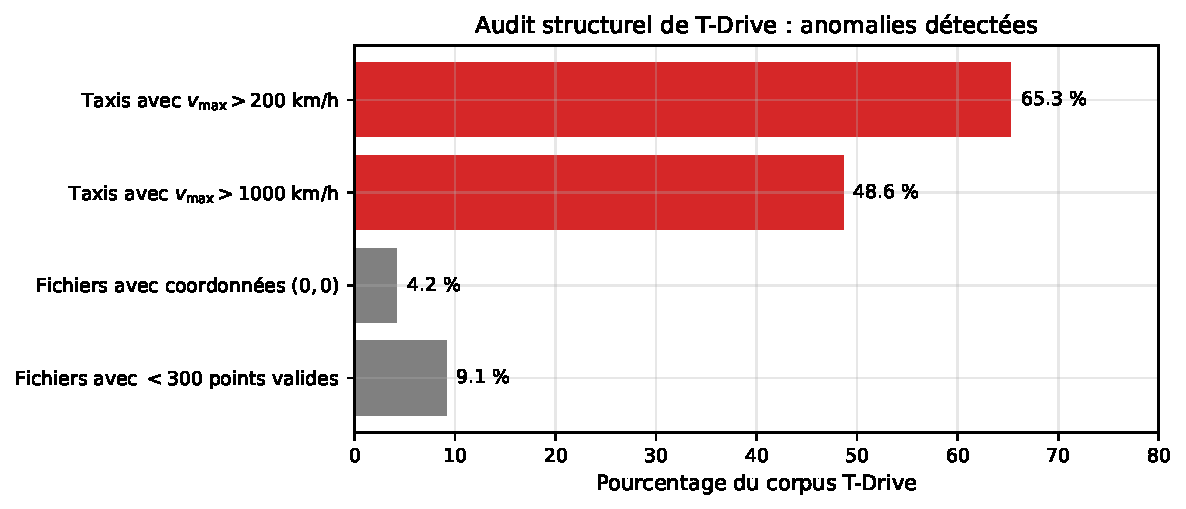
\includegraphics[width=0.85\textwidth]{graphe_6_tdrive.pdf}
\caption{Audit structurel de T-Drive. 65{,}3~\% des 10\,289 taxis présentent des vitesses
maximales supérieures à $200$~km/h et 48{,}6~\% dépassent $1\,000$~km/h : ces valeurs
sont incompatibles avec un trafic urbain. Ces artefacts rendent T-Drive inutilisable
pour l'estimation de $H$ sur la série des distances inter-points.}
\label{fig:tdrive}
\end{figure}

La figure~\ref{fig:tdrive} en donne la version visuelle : les deux premières barres sont
rédhibitoires. Une inspection manuelle de 10 fichiers confirme ces chiffres. Le fichier
\code{log_segment_0.txt} du taxi 6275 montre des sauts de 1\,495~km (Sichuan) sans
déplacement physique, avec des vitesses instantanées de $5{,}38 \times 10^6$~km/h. À
$T_{\mathrm{gap}}=900$~s, la taille médiane des segments T-Drive est de 10 points ; même à
1\,800~s, elle n'atteint que 21 points.

\begin{resultat}[T-Drive incompatible avec $H$]
T-Drive est structurellement incompatible avec l'estimation de $H$ sur la série des
distances $d_i$. Cette conclusion est \emph{factuelle} : elle repose sur le calcul et non
sur une affirmation de la littérature. L'utilisation de T-Drive pour d'autres analyses
(temps de séjour, lois de puissance) reste possible et n'a pas été testée ici.
\end{resultat}

\paragraph{T-Drive pour les lois de puissance.} Le même corpus a été testé pour
l'analyse des lois de puissance. Les fichiers T-Drive ont été convertis au format
interne (\code{sortie_tdrive/}) après filtrage des taxis à pas médian aberrant
(pas $\in [30{,}700]$~s) : 9\,307 taxis sur 10\,357 sont retenus, pour 17,6 millions
de points. Le pipeline standard (jeu 200~m~/~20~min, identique à GeoLife) détecte
165\,591 séjours et 126\,601 paires de distances.

\begin{resultat}[T-Drive inutilisable pour les lois de puissance]
La distribution des durées de séjour est dominée par les stationnements nocturnes.
Le seuil $x_{\min}$ ajusté par la méthode de Clauset est de 12{,}7~h, et la queue
ne contient que 1{,}8~\% des séjours (2\,018 sur 110\,521). Un test complémentaire
avec \code{ARRET_DUREE_MIN_S = 300~s} aggrave le phénomène : la queue tombe à
0{,}06~\% des séjours (2\,063 sur 3\,186\,489), et $x_{\min}$ reste à 12{,}6~h.
Quant aux distances, le $x_{\min}$ ajusté est de 16{,}5~km : la queue mesure des
courses entières de taxi, pas des déplacements entre activités. Dans les deux cas,
le fit est rejeté ($p_{\text{boot}} < 0{,}001$) et l'exposant ajusté ($\alpha = 4{,}9$
pour les séjours, $2{,}8$ pour les distances) ne décrit pas la mobilité humaine.
\textbf{T-Drive mesure l'exploitation d'une flotte, pas la mobilité résiduelle.}
\end{resultat}

\section{Récapitulatif des chiffres de référence}

Sauf mention contraire, tous les résultats présentés dans ce mémoire sont produits avec
la configuration \code{TIME_GAP_THRESHOLD = 900}, \code{MIN_POINTS = 300}, sur
GeoLife. Le tableau~\ref{tab:corpus} donne les chiffres de référence.

\begin{table}[ht]
\centering
\caption{Chiffres de référence du corpus analysé.}
\label{tab:corpus}
\small
\begin{tabular}{lr}
\toprule
Indicateur & Valeur \\
\midrule
Utilisateurs avec au moins un segment retenu & 145 \\
Segments retenus & 19\,150 \\
Segments gardés (critère strict) & 7\,853 (41,0~\%) \\
Utilisateurs avec au moins un segment gardé & 136 \\
Utilisateurs sans aucun segment gardé & 9 \\
Concentration des segments gardés (top 5 utilisateurs) & 25,4~\% \\
\bottomrule
\end{tabular}
\end{table}

\paragraph{Distinction des populations « gardé » et « arrêt ».}
Le chiffre « 136 utilisateurs avec au moins un segment gardé » (critère H) et le chiffre
« 137 utilisateurs avec au moins un arrêt détecté » (utilisé pour les lois de puissance)
désignent \textbf{deux populations différentes} : le premier dépend du filtre de fiabilité
sur $H$ (section~\ref{sec:circularite}) ; le second dépend de
\code{ARRET_DUREE_MIN_S = 1200~s}. Les deux ensembles diffèrent à la fois en composition
et en taille (136 vs 137).

% =====================================================================
\chapter{Pipeline de prétraitement}
\label{ch:prep}
% =====================================================================

\section{Principes de conception}

\begin{enumerate}
  \item \textbf{Marquer avant de décider.} Les points suspects sont signalés dans les
  fichiers de sortie sans être retirés ; l'effet d'une coupure est mesuré à part.
  \item \textbf{Seuils relatifs au contexte du segment (V5).} Une alternative est ajoutée
  comme variante mesurée, jamais comme remplacement silencieux.
  \item \textbf{Deux versions de chaque estimateur} : référence lisible et vectorisée,
  avec des tests de parité.
  \item \textbf{Traçabilité.} Chaque ligne porte une empreinte des constantes de
  configuration ; les simulations utilisent une graine dérivée.
\end{enumerate}

\section{Migration V4\texorpdfstring{$\to$}{->}V5 : seuils relatifs}

La V5 remplace les seuils absolus de la V4 par des grandeurs calculées localement, par
segment, bornées par des planchers/plafonds absolus. Le tableau~\ref{tab:migration}
résume les principaux changements.

\begin{table}[ht]
\centering
\caption{Migration V4$\to$V5 des filtres de marquage.}
\label{tab:migration}
\small
\begin{tabular}{p{4.2cm}p{8.5cm}}
\toprule
\textbf{Composant} & \textbf{V5} \\
\midrule
Filtre distance & $\text{seuil} = \min(30 \times \tilde d,\; 500)$ (m) \\
Filtre vitesse max & $\text{seuil} = \max(200,\; \max(5,\; 20 \times \tilde v))$ (km/h) \\
Filtre variation brutale & $\max(20,\; 5 \times \mathrm{MAD}_v)$ \\
Filtre persistance régime & $\max(5,\; \mathrm{round}(0{,}01 N))$ \\
Fallback MAD$=0$ & $\max(5,\; 3 \tilde v)$ \\
Test de stationnarité & Test KS 2-échantillons sur les deux moitiés \\
Alias log & $\max(5,\; 2{,}5 \times \text{pas médian})$ \\
\bottomrule
\end{tabular}
\end{table}

\paragraph{Volume de marquage en V5.} Sur le corpus (145 utilisateurs, 19\,150
segments retenus, 21\,960\,883 points), les filtres de la V5 marquent :
\begin{table}[ht]
\centering
\caption{Volume de points marqués par les filtres de la V5.}
\label{tab:marquage-v5}
\small
\begin{tabular}{lrr}
\toprule
Marquage & Points marqués & Fraction du corpus \\
\midrule
\code{suspect_dist}    & 148\,203 & 0,67~\% \\
\code{suspect_vitesse} & 273\,499 & 1,25~\% \\
\bottomrule
\end{tabular}
\end{table}

L'augmentation du nombre de marquages par rapport aux seuils absolus de la V4 est
\emph{attendue} par construction : le seuil de distance devient relatif à la médiane du
segment. Le nombre de segments retenus (19\,150) reste compatible avec la V4 parce que
le filtre final sur \code{MIN_POINTS} est indépendant du marquage.

\section{Calibration de \code{TIME_GAP_THRESHOLD} et \code{MIN_POINTS}}

La littérature ne fournit pas de seuil unique pour la segmentation temporelle des
trajectoires GPS. Nous avons mesuré l'impact de chaque couple (gap, $N_{\min}$) sur le
corpus, en évaluant le pourcentage de points conservés.

\begin{figure}[ht]
\centering
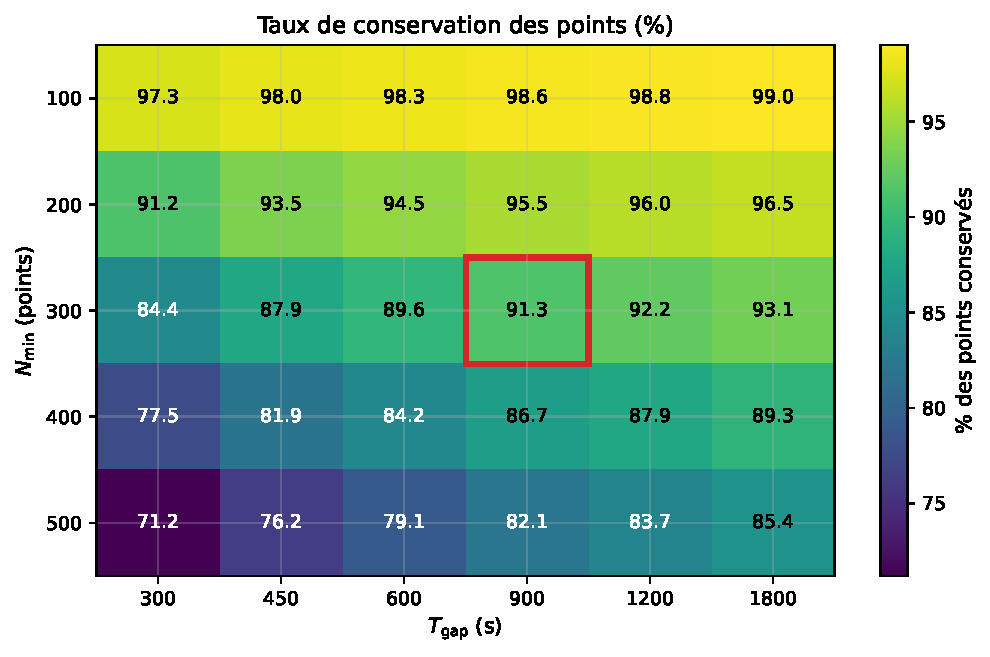
\includegraphics[width=0.8\textwidth]{graphe_5_heatmap.pdf}
\caption{Taux de conservation des points (\%) en fonction du seuil de segmentation
$T_{\mathrm{gap}}$ et du minimum de points $N_{\min}$. Le couple retenu $(900, 300)$
est dans une zone de $91{,}3\,\%$ de conservation, entouré de valeurs proches
($89{,}6$ à $600$~s, $92{,}2$ à $1\,200$~s). Cette continuité indique que la décision
n'est pas sensible à de petites variations.}
\label{fig:heatmap}
\end{figure}

\begin{figure}[ht]
\centering
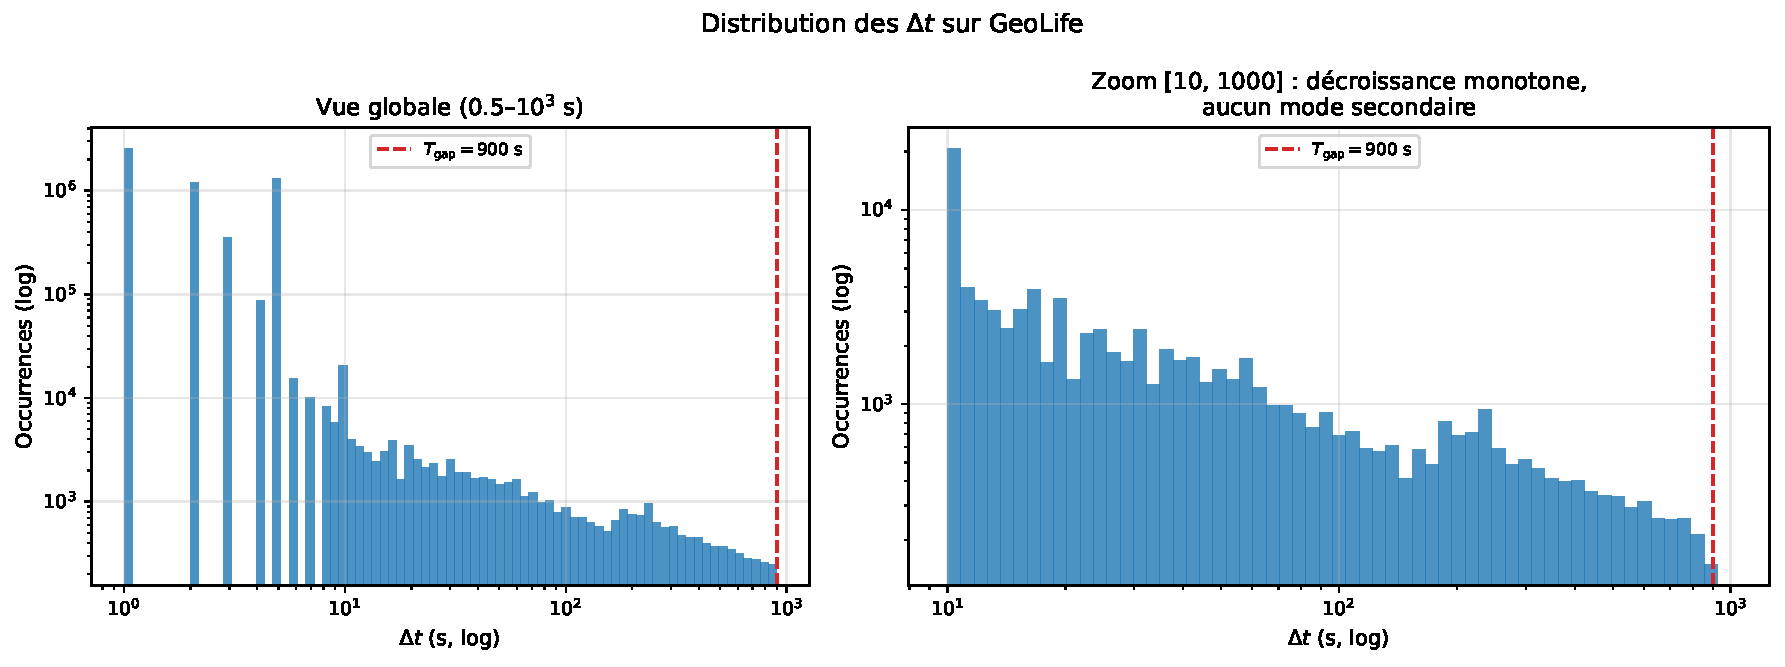
\includegraphics[width=\textwidth]{graphe_8_deltas.pdf}
\caption{Distribution des intervalles $\Delta t$ entre points successifs sur GeoLife
(échelle log-log). Les pics à 1--10~s correspondent à la résolution native des
timestamps (seconde). Au-delà de 10~s, la distribution est monotone décroissante, sans
mode secondaire. Le choix de $T_{\mathrm{gap}} = 900$~s est donc un choix externe,
calibré empiriquement (figure~\ref{fig:heatmap}), et non dicté par la structure des
données.}
\label{fig:deltas}
\end{figure}

\paragraph{Distribution des $\Delta t$.} Sur GeoLife, la distribution des écarts temporels
(figure~\ref{fig:deltas}) présente un pic à 1--10~s correspondant à la résolution native
des timestamps, puis une décroissance monotone au-delà. \emph{Il n'existe aucun pic
naturel} justifiant un seuil particulier : toute valeur doit être justifiée par une
contrainte externe.

\begin{choix}[Seuils retenus]
La figure~\ref{fig:heatmap} synthétise cette calibration. Nous avons fixé
$T_{\mathrm{gap}}=900$~s et $N_{\min}=300$ : à ce point, 91,3~\% des points sont
conservés dans des segments satisfaisant les deux critères, et la taille médiane des
segments retenus est de 721 points (figure~\ref{fig:longueurs}). Le seuil de 300 points
est le minimum empirique observé pour une régression DFA stable sur au moins cinq
échelles ; le seuil de 900~s ne fragmente pas les trajectoires en segments de quelques
minutes, tout en restant bien en-dessous des trous d'enregistrement typiques de GeoLife
(plusieurs heures à plusieurs jours).
\end{choix}

\begin{limite}
Le choix 900/300 est une décision d'ingénierie fondée sur ces chiffres, pas une
recommandation issue de la littérature. Un choix alternatif à 600/200 serait tout aussi
défendable, avec un profil différent (plus de segments, moins de fiabilité DFA par
segment).
\end{limite}

\section{Lecture, nettoyage, tri et doublons}

Les six lignes d'en-tête sont ignorées. La date et l'heure sont converties en secondes
UNIX \emph{en UTC} (cohérentes avec les labels GeoLife). Un point est rejeté si sa
latitude n'est pas dans $[-90,90]$ ou sa longitude hors de $[-180,180]$. L'ordre est :
nettoyage, tri par horodatage, puis suppression des doublons (premier conservé).

\begin{limite}
Si deux positions distinctes portent le même horodatage, la seconde est perdue. La
documentation de la fonction décrit le critère comme « même position et même horodatage »,
alors que seul l'horodatage est testé.
\end{limite}

\section{Segmentation par trous temporels}

Un trou $t_i-t_{i-1} > T_{\mathrm{gap}} = 900$~s ouvre un nouveau segment. Aucune
interpolation n'est effectuée et les segments ne sont jamais raccordés.

\begin{choix}[Couper sans raccorder]
Combler un trou ou raccorder deux morceaux fabrique un saut artificiel dans la série des
distances, auquel la DFA est très sensible~\cite{chen2002}.
\end{choix}

\begin{limite}
Le seuil de 900~s est calibré sur GeoLife (section~\ref{ch:prep}), mais reste une valeur
absolue : il n'a pas été testé sur T-Drive (où la médiane native est 300~s) ni sur
d'autres corpus.
\end{limite}

\section{Statistiques de segment et indicateurs}

Pour un segment de $N$ points, on calcule $d_i$ (Haversine), $\delta_i=t_i-t_{i-1}$ et
$v_i=d_i/(\delta_i/3600)$ en km/h. Les statistiques descriptives sont calculées en une
passe vectorisée. Deux indicateurs sont dérivés : $R = \sigma_v/\tilde v$
(hétérogénéité) et $\rho = \bar d_2/\bar d_1$ (ratio, conservé pour l'affichage
seulement).

\begin{choix}[Test de stationnarité par KS]
La V5 remplace le ratio $\rho$ (avec ses seuils $[0{,}7; 1{,}4]$) par un test de
Kolmogorov--Smirnov à deux échantillons entre les deux moitiés de la série des distances.
Le ratio est conservé pour l'affichage dans les logs (indicateur rapide à l'œil), mais il
ne pilote plus la décision.
\end{choix}

\begin{limite}[Puissance du test KS]
Le test KS détecte les décalages de distribution, mais sa puissance dépend de $N$ et de
la forme des distributions. Pour une série stationnaire à mémoire longue, la variance de
la moyenne empirique décroît comme $N^{2H-2}$, plus lentement que $N^{-1}$, et les deux
moitiés peuvent s'écarter davantage que sous l'indépendance. Le test peut donc rejeter la
stationnarité pour une série stationnaire persistante, c'est-à-dire pour le cas étudié.
Sur le corpus, \code{statio_p_value} est inférieure à $10^{-20}$ sur la quasi-totalité
des segments gardés, ce qui rend l'indicateur peu discriminant.
\end{limite}

\section{Marquage des points suspects}

\subsection{Filtre de distance}

Un point est marqué \code{suspect_dist} si $d_i>d_{\max}$, avec
$d_{\max}=\min(30 \times \tilde d, 500)$~m. Ce filtre détecte les sauts de position
grossiers, indépendamment de la vitesse.

\subsection{Filtre de vitesse par Z-score modifié}

On utilise le Z-score modifié d'Iglewicz et Hoaglin~\cite{iglewicz1993} :
$Z_i = 0{,}6745\,(v_i-\tilde v)/\mathrm{MAD}$, avec $\mathrm{MAD}=\mathrm{med}(|v_i-\tilde v|)$.
Un point est candidat si $Z_i>3{,}5$ (seuil normalisé par le MAD, non ajustable). Le
calcul est \emph{asymétrique} : seules les vitesses supérieures à la médiane sont
candidates. Un garde-fou absolu ($v>200$~km/h en plancher) classe en \code{artefact}.

\subsection{Classification des points candidats}

Chaque candidat est classé selon sa variation locale $\Delta v$ et sa persistance
(nombre de points consécutifs au-dessus du seuil).

\begin{table}[ht]
\centering
\caption{Classification des points candidats.}
\label{tab:classes}
\small
\begin{tabular}{@{}lll@{}}
\toprule
Variation $\Delta v$ & Persistance & Classe \\
\midrule
brutale ($>5 \times \mathrm{MAD}_v$) & isolée ($<5$ points) & \code{artefact} \\
quelconque & soutenue ($\ge5$ points) & \code{regime} (premier seul marqué) \\
modérée & isolée & non marqué \\
\bottomrule
\end{tabular}
\end{table}

\begin{choix}[Distinguer artefact et régime]
Un pic brutal et isolé est probablement une erreur de mesure ; une vitesse élevée qui dure
est un changement réel de comportement. Seuls les points \code{artefact} et
\code{suspect_dist} servent de points de coupure dans la variante
$\hat H_{\mathrm{morceaux}}$. Les points \code{regime} ne sont jamais des points de
coupure.
\end{choix}

\section{Sélection finale des segments}

Deux filtres retiennent les segments exploitables : au moins $N_{\min}=300$ points et une
distance parcourue d'au moins $0{,}1$~km (avec un mode relatif en option V5). La
figure~\ref{fig:longueurs} montre que ce seuil coupe une minorité de segments (66~\% des
segments retenus ont moins de 1\,000 points), mais la médiane à 721 points reste
en-dessous des 2\,500 points recommandés par la littérature (Eke et al., 2002) — cette
limite est assumée.

\subsection{Distribution des longueurs}

\begin{figure}[ht]
\centering
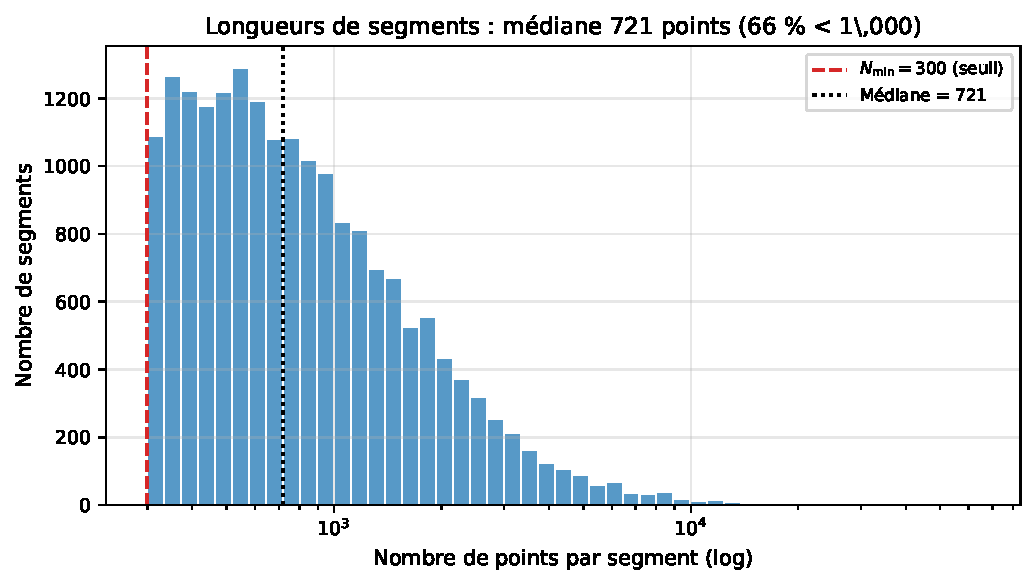
\includegraphics[width=0.75\textwidth]{graphe_7_longueurs.pdf}
\caption{Distribution des longueurs de segments retenus (échelle log). La médiane est
de 721 points, très au-dessus du seuil $N_{\min} = 300$. 66~\% des segments ont moins
de $1\,000$ points. Le seuil $N_{\min}=300$ coupe une minorité, mais reste en-dessous
des 2\,500 points recommandés par la littérature pour une estimation stable de $H$.}
\label{fig:longueurs}
\end{figure}

\begin{limite}
Le seuil de 300 points a un sens physique différent selon le mode d'enregistrement
(5~minutes à 1~s, 50~minutes à 10~s). Ces filtres s'appliquent \emph{avant} la détection
d'arrêts : les segments courts, et les segments quasi immobiles où un long séjour a été
enregistré, sont absents de l'analyse des temps de séjour.
\end{limite}

\begin{limite}[Biais de sélection sur les lois de puissance]
Sur le corpus, \code{MIN_POINTS = 300} exclut 37 utilisateurs sur 183 (20~\%),
représentant des profils variés (segments trop courts : 148, 32, 180, 235, \dots{} points
maximaux ; ou points insuffisants : 17, 81, 152, 199, \dots). Ce seuil est justifié pour
la stabilité de DFA, mais \textbf{n'a aucune justification pour l'analyse des lois de
puissance} : un utilisateur avec un segment maximal de 148 points peut avoir plusieurs
arrêts et distances exploitables. L'effet de cette exclusion sur l'exposant $\alpha$
agrégé n'a pas été quantifié.
\end{limite}

\section{Mode d'enregistrement}

L'heuristique classe un fichier en mode \emph{temps} si au moins 60~\% des pas ont un
intervalle à $\pm 20$~\% de la médiane, et en mode \emph{distance} si au moins 50~\% des
pas en mouvement ont une distance à $\pm 30$~\% de la médiane. Le mode peut changer à
l'intérieur d'un fichier.

\section{Traçabilité}

Chaque ligne de résultats porte une empreinte (\code{empreinte_config}) des réglages.
Changer une seule constante change l'empreinte. Les tableaux de validation sont générés
par script.

% =====================================================================
\chapter{Détection d'arrêts et temps de séjour}
\label{ch:arrets}
% =====================================================================

\section{Variables étudiées}

Le module \code{arrets.py} construit deux variables : le \emph{temps de séjour} et la
\emph{distance entre deux arrêts consécutifs}.

\section{Algorithme}

On utilise une fenêtre ancrée, selon Li et al.~\cite{li2008} employé sur des trajectoires
GPS dans~\cite{zheng2009}. Pour chaque point $p_i$ pris comme ancre, soit $j$ le premier
indice tel que $\mathrm{dist}(p_i,p_j)>R_{\mathrm{arr}}$. Si $t_j-t_i\ge T_{\min}$, on
déclare un arrêt localisé au centroïde. Les valeurs retenues sont
$R_{\mathrm{arr}}=200$~m et $T_{\min}=1200$~s (20~min), conformément à l'école Zheng et
al. adaptée à GeoLife. Quatre couples $(R_{\mathrm{arr}}, T_{\min})$ sont testés en
sensibilité : $(100, 300)$, $(100, 600)$, $(200, 1200)$, $(200, 1800)$.

\begin{choix}[Suivre Zheng plutôt que Li]
Deux écoles coexistent dans la littérature GPS : 100~m~/~5~min (trackintel) et
200~m~/~20--30~min (Zheng et al.). GeoLife étant le corpus de référence de Zheng, nous
suivons la seconde. La sensibilité au couple est mesurée via
\code{ARRET_JEUX_SENSIBILITE}.
\end{choix}

\section{Observation finie et censure}
\label{sec:censure}

Suivant Kivelä et Porter~\cite{kivela2015}, le code n'écarte pas les durées biaisées :
il les étiquette (colonne \code{censuree}). Un arrêt qui commence au premier point d'un
morceau est \emph{censuré à gauche}. Un arrêt jamais suivi d'une sortie du rayon n'est pas
détecté par défaut, sauf option \code{inclure_dernier}. Les \emph{pauses entre segments}
sont récupérées à part, avec le type \code{entre_segments}.

\begin{choix}[Exclure les séjours censurés par défaut]
Pour l'ajustement, on ne garde que les arrêts internes non censurés.
\end{choix}

\section{Distances entre arrêts}

Les distances entre arrêts consécutifs sont calculées à l'intérieur d'un même segment, et
celles inférieures à 100~m sont écartées.

\paragraph{Deux variantes de distance.} Le code distingue deux variables :
\begin{itemize}
\item \code{distance} : uniquement les paires dont les deux arrêts sont \emph{dans le
même segment} (aucun trou entre eux). C'est la variante « propre ».
\item \code{distance_a_cheval} : aussi les paires séparées par un trou d'enregistrement.
C'est la variante « large ».
\end{itemize}
Le compromis est discuté au chapitre~\ref{ch:lp-resultats} : la restriction « même
segment » élimine environ 90~\% des paires sur le corpus (1283 sur 11499), ce qui rend la
variante propre peu exploitable statistiquement.

\section{Limites connues}

\begin{limite}[Filtres en amont]
La détection s'exécute sur les segments retenus. Les segments courts et quasi immobiles
sont absents : les séjours sont sélectionnés selon la longueur du segment qui les contient.
\end{limite}

\begin{limite}[Fragmentation d'un séjour]
Le bruit GPS peut faire sortir un point du rayon et couper artificiellement un long séjour
en deux. Le second morceau est tronqué, sans étiquetage censuré. Cet effet fausse la
queue de la distribution des durées, précisément ce que l'on cherche à estimer.
\end{limite}

\begin{limite}[Durées surestimées]
La durée inclut le pas de sortie du rayon, surtout près de $T_{\min}$.
\end{limite}

% =====================================================================
\chapter{Estimation de $H$ par segment et filtre de fiabilité}
\label{ch:est}
% =====================================================================

\section{Implémentation en double version}

Les trois estimateurs sont implémentés en deux versions (référence / vectorisée), avec
tests de parité. La série d'entrée est $d_1,\dots,d_{N-1}$
(\code{SERIE_ANALYSEE="distance"}). L'option \code{--serie vitesse} analyse les $v_i$ à
titre de contrôle.

\begin{choix}[Série des distances]
La série des $d_i$ est imposée par le cahier des charges. Son défaut est de mélanger
vitesse et intervalle de temps ($d_i=v_i\delta_i$). Elle mesure l'intensité du déplacement
et non sa direction.
\end{choix}

\section{Paramètres des estimateurs}

La DFA utilise 20 échelles de $s_{\min}=4$ à $\lfloor N/4\rfloor$. Le code calcule aussi
les pentes des moitiés basse et haute (\code{dfa_bas}, \code{dfa_haut}), leur écart
(\code{ecart_pentes}), et des pentes locales sur fenêtres de 5 échelles. Le R/S utilise
des blocs de 10 à $\lfloor N/2\rfloor$. Le Whittle local utilise
$m=\min(\lfloor N^{0,65}\rfloor, \lfloor N/4\rfloor)$ fréquences et la grille de la
section~\ref{sec:whittle}.

\section{Colonnes de sortie et drapeaux de fiabilité}

Le script \code{03_estimation_H.py} écrit, pour chaque segment, $\hat H$ par chaque
méthode (dont \code{h_rs_corrige}) et des colonnes de fiabilité :
\code{dfa_sup_1}, \code{whittle_m}, \code{whittle_a_la_borne},
\code{nul_p}, \code{nul_seuil}, \code{nul_exces}, \code{nul_ordre_ar},
\code{mode_echantillonnage}. Le script calcule aussi la \emph{divergence} entre méthodes
(écart entre l'estimation maximale et minimale disponibles) et le flag \code{suspect}
au-delà de $0{,}15$.

\section{Le filtre de fiabilité \code{04_H_valides.py}}

Un segment est \emph{gardé} si et seulement si les quatre conditions suivantes sont
vérifiées :
\begin{enumerate}
  \item les trois méthodes ont produit une valeur (ni NaN ni absente) ;
  \item $0 < \hat H_{\mathrm{DFA}} < 1$, $0 < \hat H_{\mathrm{RS}} < 1$,
  $0 < \hat H_{\mathrm{Whittle}} < 1$ ;
  \item \code{whittle_a_la_borne = False} (le minimum de $R(H)$ n'est pas à la borne
  de la grille) ;
  \item \code{divergence} $\le 0{,}15$.
\end{enumerate}
Les segments gardés sont sauvegardés dans \code{resultats_H_valides/<user>_H_gardes.csv},
avec une colonne \code{fort_0p5} indiquant si les trois méthodes donnent $H>0{,}5$.

\begin{resultat}[Chiffres de référence sur le corpus GeoLife]
Sur 19\,150 segments retenus et 145 utilisateurs, 7\,853 segments sont gardés
(41,0~\%). Parmi eux, la quasi-totalité (97,1~\%) est également \emph{forte}, c'est-à-dire
avec les trois méthodes $>0{,}5$.
\end{resultat}

\section{Critique de la circularité du filtre}
\label{sec:circularite}

\begin{limite}[Circularité de la sélection]
Le filtre de fiabilité porte sur le résultat lui-même. La condition
\code{divergence} $\le 0{,}15$ utilise les valeurs de $\hat H$ des trois méthodes, et les
conditions de bornes utilisent également $\hat H$. L'écart moyen
$|\hat H_{\mathrm{DFA}} - \hat H_{\mathrm{RS}}|$ passe de $0{,}079$ sur l'ensemble des
utilisateurs à $0{,}023$ sur les utilisateurs gardés (moyenne par utilisateur). Le même
calcul mené par segment donne $0{,}152 \to 0{,}058$ : la réduction est du même ordre. Dans
les deux cas, elle est \emph{par construction}, et non une confirmation indépendante de la
convergence des méthodes. Le $\hat H_{\text{gardés}}$ doit donc être lu comme un $\hat H$
\textbf{conditionnel au filtre}, et non comme un $\hat H$ de population.
\end{limite}

\begin{figure}[ht]
\centering
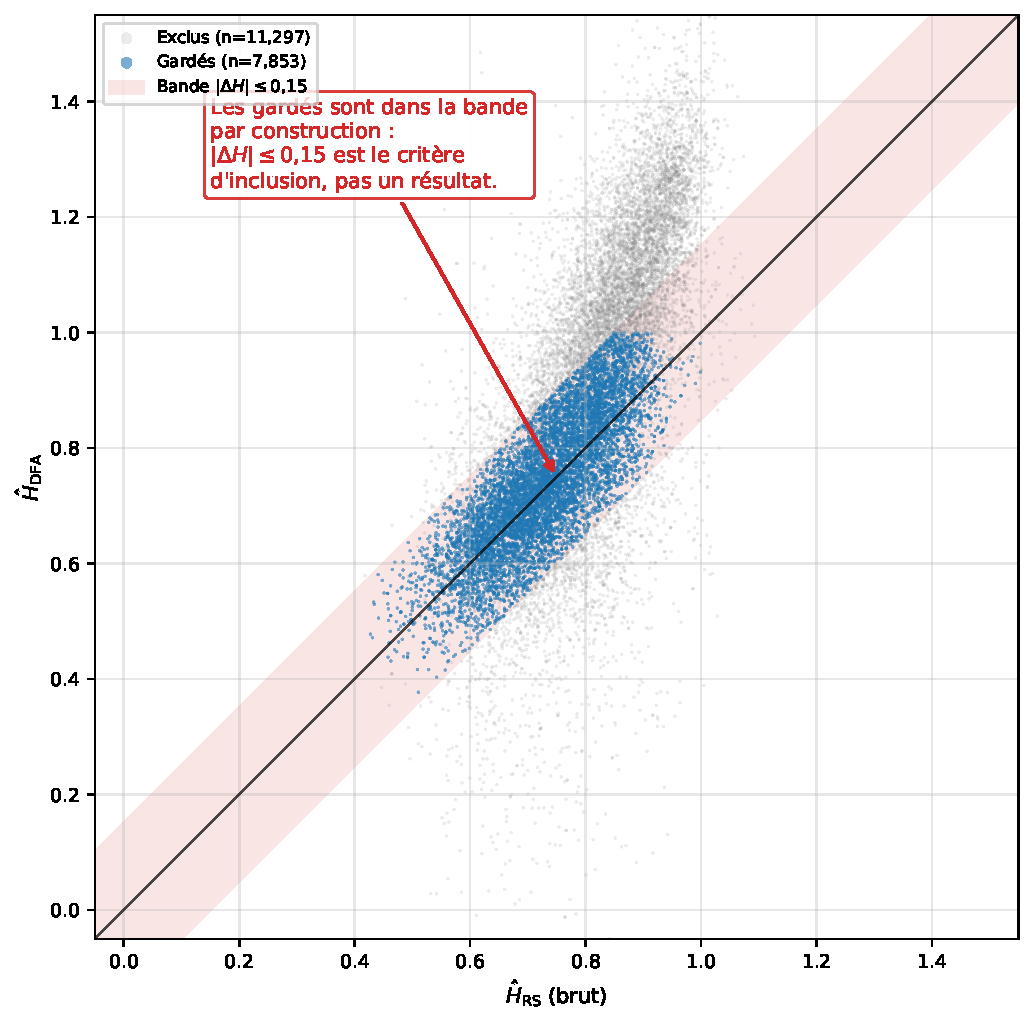
\includegraphics[width=0.75\textwidth]{graphe_3_circularite.pdf}
\caption{$\hat H_{\mathrm{DFA}}$ contre $\hat H_{\mathrm{RS}}$ pour tous les segments,
coloriés selon le critère de garde. Les segments gardés sont concentrés dans la bande
$|\Delta H| \leq 0{,}15$ \emph{par construction} : cette bande est le critère
d'inclusion, non un résultat de la convergence indépendante des méthodes. La convergence
des gardés ne peut donc pas être invoquée comme preuve indépendante.}
\label{fig:circularite}
\end{figure}

Cette limite est la plus importante du mémoire. La figure~\ref{fig:circularite} la rend
immédiatement visible : les points gardés sont concentrés dans la bande
$|\Delta H| \leq 0{,}15$ non parce que les méthodes sont indépendamment d'accord, mais
parce que la bande est le critère de sélection. Le $\hat H_{\text{gardés}}$ doit donc
être lu comme un $\hat H$ conditionnel au filtre, non comme un $\hat H$ de population.

\section{Variante par morceaux}

$\hat H_{\mathrm{morceaux}}$ est $\hat H_{\mathrm{DFA}}$ calculé après coupure du segment
aux points \code{artefact} et \code{suspect_dist}, sans raccord, puis combiné par moyenne
pondérée par la longueur des morceaux (taille minimale d'un morceau : 50 points).

% =====================================================================
\chapter{Validation synthétique et hypothèses}
\label{ch:valid}
% =====================================================================

\section{Générateur de bruit gaussien fractionnaire}

Les séries de $H$ connu sont générées exactement par plongement circulant de la covariance,
selon Davies et Harte~\cite{davies1987}. Un fBm s'obtient par somme cumulée du fGn. Des
modèles à mémoire courte (AR(1), moyenne à changements de régime) et un processus ON/OFF à
durées de Pareto complètent le catalogue.

\section{Exactitude des estimateurs}
\label{sec:exactitude}

Le script \code{02_validation_methodes.py} génère, pour chaque couple $(H_0,N)$, un
nombre fixé de réalisations d'un fGn, estime $H$ par quatre variantes et résume le biais
et l'erreur quadratique moyenne (RMSE). Le tableau~\ref{tab:exactitude} donne les cellules
pertinentes pour l'interprétation du corpus.

\begin{figure}[ht]
\centering
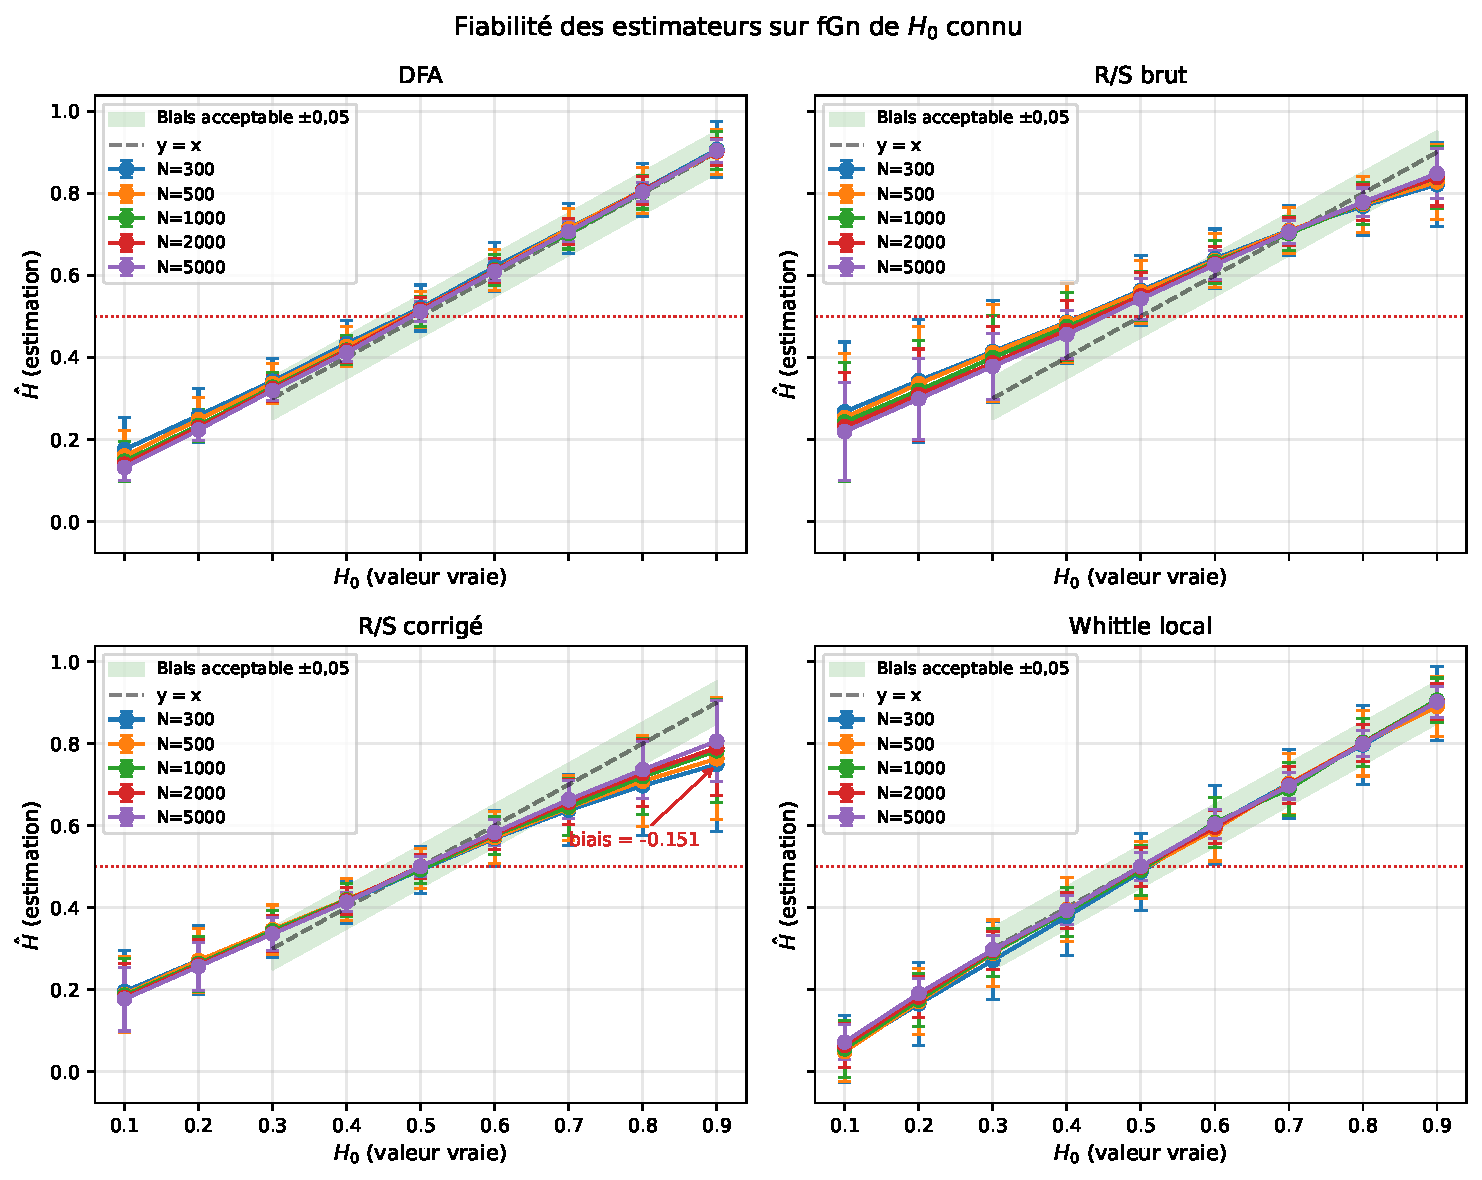
\includegraphics[width=\textwidth]{graphe_1_validation.pdf}
\caption{Biais et RMSE des quatre variantes d'estimation sur des fGn de $H_0$ connu
(200 répliques par cellule). DFA et Whittle suivent la diagonale ; le R/S corrigé
(Anis--Lloyd) sous-estime les séries persistantes au-delà de $H_0 = 0{,}7$
(biais $-0{,}149$ à $N=300$, $H_0=0{,}9$). Ce biais mesuré justifie de ne pas
utiliser R/S comme référence indépendante pour valider un $H$ élevé.}
\label{fig:validation}
\end{figure}

\begin{table}[ht]
\centering
\caption{Biais et RMSE des estimateurs sur fGn de $H_0$ connu (200 réalisations par cellule, graine 20261018).}
\label{tab:exactitude}
\small
\begin{tabular}{rrrrrrrrr}
\toprule
$H_0$ & $N$ & \multicolumn{2}{c}{DFA} & \multicolumn{2}{c}{R/S corrigé} & \multicolumn{2}{c}{Whittle} \\
 & & biais & RMSE & biais & RMSE & biais & RMSE \\
\midrule
0{,}5 & 300 & $+0{,}032$ & $0{,}065$ & $+0{,}004$ & $0{,}056$ & $+0{,}002$ & $0{,}091$ \\
0{,}7 & 300 & $+0{,}011$ & $0{,}061$ & $-0{,}065$ & $0{,}093$ & $-0{,}000$ & $0{,}095$ \\
0{,}9 & 300 & $+0{,}011$ & $0{,}067$ & $-0{,}149$ & $0{,}161$ & $-0{,}002$ & $0{,}081$ \\
0{,}7 & 1000 & $+0{,}007$ & $0{,}039$ & $-0{,}048$ & $0{,}063$ & $-0{,}001$ & $0{,}059$ \\
0{,}9 & 1000 & $+0{,}002$ & $0{,}045$ & $-0{,}121$ & $0{,}127$ & $+0{,}001$ & $0{,}052$ \\
\bottomrule
\end{tabular}
\end{table}

\paragraph{Conséquences.} DFA et Whittle sont fiables sur l'ensemble du domaine
$H \in [0{,}3, 0{,}9]$ (RMSE $\le 0{,}067$ à $N=300$, $\le 0{,}060$ à $N=1000$). R/S
corrigé est fiable à $H \le 0{,}5$ mais devient inutilisable comme référence pour
$H \ge 0{,}7$ : la correction Anis--Lloyd sur-corrige les séries persistantes.
\textbf{Cette conclusion est vérifiée par le calcul sur 2\,400 séries synthétiques.}
La figure~\ref{fig:validation} visualise ces résultats : la dégradation du R/S corrigé
à haute persistance y est immédiate, là où le tableau ne la montre que chiffre par
chiffre.

\section{Test de dépassement d'un modèle à mémoire courte}
\label{sec:nul}

La pente DFA observée est comparée à celles de séries à mémoire courte de même longueur
et de même distribution. La procédure est :
\begin{enumerate}
  \item transformer la série en loi normale par ses rangs ;
  \item ajuster un AR($p$) par Yule--Walker ($p\le p_{\max}$ choisi par AIC) ;
  \item simuler 99 séries AR($p$) de même longueur ;
  \item leur redonner exactement la distribution de valeurs par échange de rangs.
\end{enumerate}
La $p$-valeur est la proportion de surrogats dont la pente est au moins égale à la pente
observée, avec $+1$ au numérateur et au dénominateur. Le test est rapporté pour
$p_{\max}=1$ et $p_{\max}=5$.

\begin{limite}
Ce n'est pas un test de mémoire longue : il indique qu'une dépendance n'est pas expliquée
par un AR($p$). Une alternance de régimes la produit aussi~\cite{diebold2001}. Le test
n'est pas un argument suffisant pour conclure à de la LRD.
\end{limite}

\begin{limite}
La sémantique exacte de la colonne \code{nul_p} a été vérifiée dans le code source
(\code{validation/modeles_nuls.py}) : il s'agit d'une p-valeur unilatérale, calculée
comme $(1 + \#\{h_{\text{surr}} \ge h_{\text{obs}}\}) / (B+1)$ sur $B$ surrogats AR($p$)
avec marginale réimposée. Le test dit « non expliqué par un AR($p$) », pas « mémoire
longue ». Ce point est repris dans la discussion de H4.
\end{limite}

\section{Hypothèses testées et verdicts}
\label{sec:hypotheses}

Huit hypothèses ont été formulées puis testées, avec un seuil pré-fixé avant chaque test.
Le tableau~\ref{tab:hypotheses} rapporte les verdicts, y compris ceux qui ne sont pas des
confirmations.

\begin{table}[ht]
\centering
\caption{Hypothèses testées, seuils pré-fixés et verdicts.}
\label{tab:hypotheses}
\small
\begin{tabular}{p{0.6cm}p{4.6cm}p{2.6cm}p{5cm}}
\toprule
\textbf{Hyp.} & \textbf{Énoncé} & \textbf{Seuil pré-fixé} & \textbf{Verdict} \\
\midrule
H1 & Estimateurs fiables sur fGn & $|\text{biais}| < 0{,}05$ & DFA/Whittle confirmés, R/S infirmé à $H \ge 0{,}7$ \\
H2 & Régime $\to$ rejet du nul AR($p$) & taux de rejet $\ge 0{,}5$ & Confirmée à $N=1000$ ($p=1$ : 100~\% ; $p=5$ : 19~\%) ; partielle à $N=300$ ($p=1$ : 76~\% ; $p=5$ : 6~\%) \\
H3 & Corrélation $\rho_1$--$H$ & $|\rho_S| > 0{,}5$ & Confirmée ($\rho_S = 0{,}859$) \\
H4 & AR(1) reproduit les taux du corpus & $\Delta T < 10$~pts & Infirmée (corpus 20,3~\% ; $\phi=0{,}5$ et $\phi=0{,}8$ : 2--6~\%) \\
H5 & Mobile/non-mobile à $\rho_1$ fixé & $|\Delta| < 0{,}10$ & Confirmée mais fragile ($\Delta = +0{,}057$) \\
H6 & Test nul calibré à $\rho_1 = 0$ & $\in [0{,}03, 0{,}07]$ & Confirmée (5{,}25~\%) \\
H7 & Corpus invalide pour $H$ & fraction $< 0{,}10$ & Infirmée (82{,}9~\% valides) \\
\bottomrule
\end{tabular}
\end{table}

\paragraph{H1 : R/S n'est pas confirmée.} Sur fGn à $H_0=0{,}9$ et $N=300$, le R/S corrigé
présente un biais de $-0{,}149$ et un RMSE de $0{,}161$. La correction Anis--Lloyd,
conçue pour $H=0{,}5$, sur-corrige à haute persistance.

\paragraph{H2 : dépend de $N$ et de l'ordre $p$.} Le modèle \code{regimes} utilisé
(\code{changements_de_regime} de \code{simulation/memoire_courte.py}) est un processus
à moyennes constantes par morceaux, de paramètres figés. Il déclenche le rejet du nul à
$N=1000$ dans 100~\% des cas avec $p=1$, mais seulement 19~\% avec $p=5$ : un ordre AR
plus élevé absorbe une partie de l'autocorrélation artificielle créée par les paliers. À
$N=300$, la puissance chute (76~\% à $p=1$, 6~\% à $p=5$). La conclusion porte sur le
modèle \code{regimes} générique.

\paragraph{H4 : infirmée.} Le taux de rejet du modèle nul sur le corpus est de 20,3~\%.
Les deux seules valeurs de $\phi$ testées ($\phi=0{,}5$ et $\phi=0{,}8$) produisent
respectivement 2~\% et 3~\%, très loin du compte. Le corpus n'est donc pas explicable par
un AR(1). En revanche, ce taux de 20,3~\% est compatible avec le modèle \code{regimes}
(19~\% à $p=5$) et avec un fGn de $H=0{,}6$ (16~\% à $p=5$) : le rejet du nul est donc
cohérent avec l'hypothèse « régimes » ou « mémoire longue modérée », pas avec « iid ».

\paragraph{H6 : calibrée à $\rho_1 = 0$.} Sur le modèle iid ($\rho_1 = 0$), le taux de
faux positifs est de 5,25~\%, cohérent avec le seuil nominal $\alpha = 0{,}05$. Sur AR(1)
à $\rho_1 = 0{,}5$, le taux tombe à 2,5~\%, ce qui confirme que le test AR($p$) absorbe
une partie de la dépendance à court terme et devient plus conservateur. Ce dernier point
n'invalide pas H6 (qui porte sur $\rho_1 = 0$) mais précise le comportement du test.

\paragraph{H7 : infirmée pour cause de critère mal posé.} La fraction de segments valides
($s_{\max}/s_{\min} \ge 4$) est de 82{,}9~\%, très supérieure au seuil de 10~\%. Un
critère plus strict (une décade complète) inverserait la conclusion. L'infirmation porte
sur la formulation, pas sur le corpus.

\section{Test du mécanisme ON/OFF}

L'hypothèse de travail est que la dépendance apparente pourrait provenir d'une alternance
mouvement/arrêt à queue de Pareto (section~\ref{sec:onoff}). Le script
\code{mecanisme_on_off.py} vérifie d'abord sur données simulées que DFA et Whittle
retrouvent $H=(3-a)/2$, puis compare sur données réelles le $H$ mesuré à la prédiction
issue de l'exposant des séjours.

\begin{limite}
Dans la version actuelle, la simulation de comparaison est appelée avec deux exposants
distincts, alors que chaque lot de durées est tiré avec un seul exposant. Un correctif
tire chaque durée avec l'exposant de son état ; les résultats de la partie réelle doivent
être régénérés après correction.
\end{limite}

\section{Sensibilité au prétraitement}

L'expérience recalcule $\hat H_{\mathrm{DFA}}$ sur les mêmes segments sous plusieurs
variantes : coupure aux artefacts sans raccord, coupure aux trous de plus de 60~s,
coupure aux intervalles supérieurs à trois fois le pas médian, série des vitesses, échelle
minimale de DFA plus grande, stratification par mode d'enregistrement. Un \emph{placebo}
retire le même nombre de points que la coupure aux artefacts, à des positions aléatoires.

% =====================================================================
\chapter{Lois de puissance : méthodologie}
\label{ch:lp}
% =====================================================================

\section{Ajustement de Clauset}

Le module \code{lois_de_puissance/} implémente la méthode de Clauset et
al.~\cite{clauset2009}. Le maximum de vraisemblance de $\alpha$ est calculé pour un
$x_{\min}$ donné ; $x_{\min}$ minimise la distance de Kolmogorov--Smirnov sur au plus
200 seuils candidats, la queue devant compter au moins 50 points. L'adéquation est testée
par un bootstrap semi-paramétrique (1\,000 simulations). La loi est \emph{rejetée} si la
$p$-valeur est $\le 0{,}1$.

\section{Lois alternatives}

Quatre alternatives sont ajustées sur la même queue : exponentielle, log-normale, Weibull
et loi de puissance à coupure exponentielle. Chacune est comparée à la loi de puissance
par un rapport de log-vraisemblance (test de Vuong~\cite{vuong1989}). Des poids d'Akaike
corrigés~\cite{burnham2002} complètent la comparaison.

\section{Verdict}

Chaque distribution reçoit un verdict parmi :
\code{rejetee}, \code{alternative_meilleure}, \code{plausible},
\code{insuffisant}, \code{indetermine}. « Plausible » signifie seulement que la loi n'est
pas rejetée : d'autres lois peuvent être tout aussi plausibles.

\section{Populations et domaine ON/OFF}

L'ajustement est fait sur l'ensemble des utilisateurs agrégés puis, pour chaque
utilisateur ayant au moins 100 observations, séparément. Pour chaque ajustement, le code
calcule l'exposant de survie $a=\alpha-1$ et indique si $\alpha$ est dans le domaine
$2<\alpha<3$ de la relation~\eqref{eq:onoff}.

\section{Limites connues}

\begin{limite}[Indépendance et agrégation]
Le bootstrap suppose des observations indépendantes. Les durées d'une même personne sont
probablement corrélées, et l'agrégation d'utilisateurs hétérogènes mélange des lois.
\end{limite}

\begin{limite}[Censure]
L'exclusion des durées censurées retire les plus longues et biaise l'exposant vers le
haut. La correction naturelle (vraisemblance avec censure) n'est pas implémentée.
\end{limite}

\begin{limite}[Réglages]
200 simulations de bootstrap limitent la précision de la $p$-valeur ; une queue minimale
de 50 points rend le choix de $x_{\min}$ instable pour les petits utilisateurs. Le seuil
$0{,}1$ est appliqué à de nombreux utilisateurs sans correction pour tests multiples.
\end{limite}

% =====================================================================
\chapter{Lois de puissance : résultats sur GeoLife}
\label{ch:lp-resultats}
% =====================================================================

\section{Configuration et population}

L'analyse des lois de puissance est menée sur \textbf{137 utilisateurs} de GeoLife, à
savoir ceux pour lesquels au moins un arrêt a été détecté (rappel : sur 145 utilisateurs
ayant au moins un segment retenu, huit n'ont aucune pause $\ge 1200$~s dans un rayon de
200~m — 021, 049, 102, 116, 118, 166, 170, 173 — et l'utilisateur 182 est exclu pour
cause de non-comparabilité). \textbf{Ce chiffre de 137 est distinct du chiffre de 136
« utilisateurs avec au moins un segment gardé » du critère H} (section~\ref{tab:corpus}).

Le jeu de seuils utilisé est le jeu par défaut : $R_{\mathrm{arr}} = 200$~m,
$T_{\min} = 1200$~s (20~min). Les quatre couples de \code{ARRET_JEUX_SENSIBILITE} ont
été exécutés en sensibilité (section~\ref{sec:lp-sensibilite}). Les $p$-valeurs
d'adéquation sont obtenues avec 1\,000 simulations bootstrap, et les alternatives sont
activées. L'empreinte de configuration est reportée dans le tableau~\ref{tab:lp-agrege}.

\section{Résultats agrégés}

\begin{table}[ht]
\centering
\caption{Résultats agrégés des lois de puissance sur 137 utilisateurs (jeu 200~m~/~20~min, $B=1000$).}
\label{tab:lp-agrege}
\small
\begin{tabular}{lrrrrl}
\toprule
Variable & $n$ & $\alpha$ & $p_{\text{boot}}$ & Verdict & Meilleur AICc \\
\midrule
\code{sejour} & 5\,354 & $3{,}186 \pm 0{,}031$ & $0{,}159$ & alternative meilleure & tronquée (0{,}967) \\
\code{distance} (même seg.) & 1\,283 & $2{,}026 \pm 0{,}084$ & $0{,}055$ & rejetée & loi de puissance (0{,}528) \\
\code{sejour_avec_censurees} & 13\,378 & $2{,}365 \pm 0{,}029$ & $<0{,}001$ & rejetée & loi de puissance (0{,}577) \\
\code{distance_a_cheval} & 10\,216 & $1{,}779 \pm 0{,}012$ & $<0{,}001$ & rejetée & tronquée (0{,}511) \\
\bottomrule
\end{tabular}
\end{table}

\begin{figure}[ht]
\centering
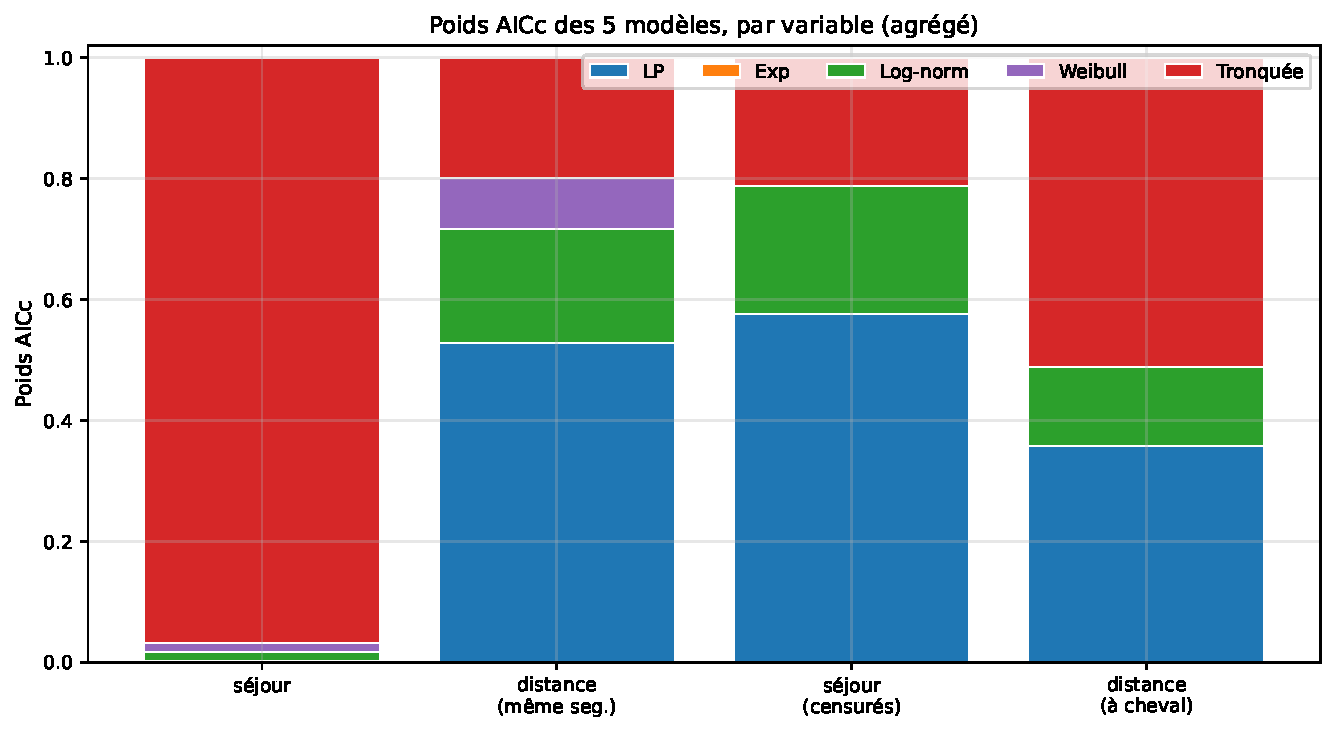
\includegraphics[width=\linewidth]{graphe_10_aicc.pdf}
\caption{Poids d'Akaike corrigés (AICc) des cinq modèles, par variable (population
agrégée, $x \geq x_{\min}$, $B = 1000$). Chaque barre somme à 1. La loi de puissance
pure (bleu) gagne pour \code{distance} (même segment) et \code{sejour_avec_censurees},
la loi tronquée (rouge) gagne pour \code{sejour} et \code{distance_a_cheval}.}
\label{fig:lp-aicc}
\end{figure}

\paragraph{Constat immédiat.} La loi de puissance pure n'est \emph{jamais} le meilleur
modèle AICc avec un poids écrasant, et elle est rejetée au seuil 0{,}1 pour trois
variables sur quatre. Pour les deux variables où la \emph{loi de puissance tronquée}
gagne (poids AICc 0{,}967 et 0{,}511), l'avantage est important ou significatif
($p_{\text{Vuong}} = 0{,}0002$ et $p_{\text{Vuong}} = 0{,}099$). Mais le modèle gagnant
n'est pas pour autant adéquat : voir le test bootstrap ci-dessous. Le poids d'AICc de
chaque modèle est reporté sur la figure~\ref{fig:lp-aicc}.

\paragraph{Adéquation de la loi de puissance pure.} La figure~\ref{fig:lp-pvalues}
reporte les $p$-valeurs du test de Clauset pour les quatre variables. Seul
\code{sejour} n'est pas rejeté ($p = 0{,}159$) ; les trois autres variables sont
rejetées. Ce test porte spécifiquement sur la loi de puissance \emph{pure}.

\begin{figure}[ht]
\centering
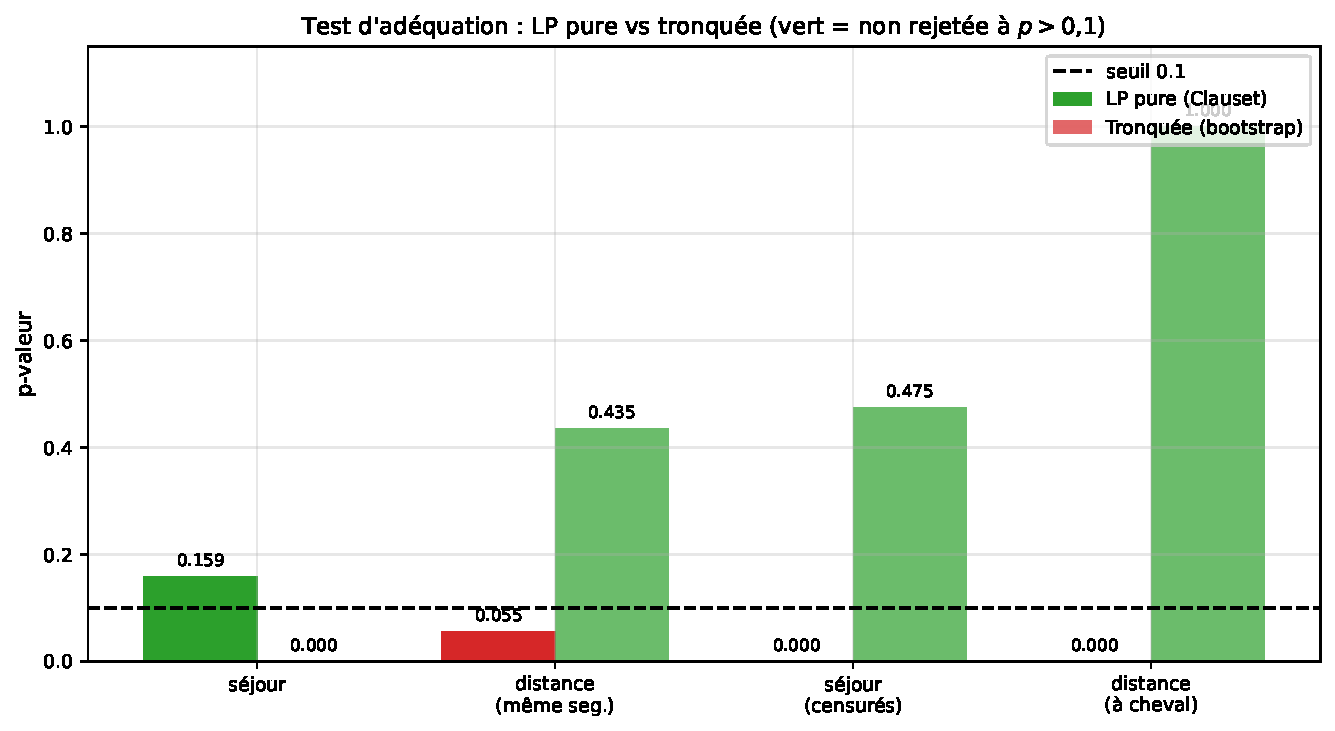
\includegraphics[width=0.85\linewidth]{graphe_11_pvalues.pdf}
\caption{Test d'adéquation de la loi de puissance pure (bootstrap de Clauset,
$x_{\min}$ ré-estimé, $B = 1000$). Vert : non rejetée à $p > 0{,}1$. Seul
\code{sejour} n'est pas rejeté ($p = 0{,}159$) ; les trois autres variables sont
rejetées. Le test d'adéquation de la loi tronquée (tableau~\ref{tab:lp-adequation})
suit une procédure différente et n'est pas directement comparable sur cette figure.}
\label{fig:lp-pvalues}
\end{figure}

\paragraph{Le modèle gagnant est-il adéquat ?} Le critère AICc compare les modèles
entre eux ; il ne dit pas si le modèle gagnant est un \emph{bon} ajustement. Un test
bootstrap d'adéquation (200 simulations, $x_{\min}$ fixé, voir la limite correspondante)
a donc été appliqué à la loi de puissance tronquée sur chaque variable.
Le tableau~\ref{tab:lp-adequation} rapporte les résultats.

\begin{table}[ht]
\centering
\caption{p-valeurs d'adéquation de la loi de puissance tronquée (bootstrap, $B=200$, $x_{\min}$ fixé).}
\label{tab:lp-adequation}
\small
\begin{tabular}{lrrl}
\toprule
Variable & $p_{\text{tronq}}$ & Verdict & Lecture \\
\midrule
\code{sejour} & $<0{,}005$ & rejetée & Aucun modèle adéquat \\
\code{distance} (même seg.) & $0{,}435$ & non rejetée & Test permissif, aucune conclusion \\
\code{sejour_avec_censurees} & $0{,}475$ & non rejetée & $\lambda \approx 0$ (loi de puissance pure) \\
\code{distance_a_cheval} & $1{,}000$ & non rejetée & Artefact ($\lambda \to 0$) \\
\bottomrule
\end{tabular}
\end{table}

Deux cas sont informatifs :
\begin{itemize}
\item \code{sejour} : la tronquée est \textbf{rejetée} à $p<0{,}005$, malgré le fait
que le test soit peu puissant (limite en fin de chapitre). C'est un rejet robuste.
\textbf{Aucun des cinq modèles n'est adéquat pour les durées de séjour.}
\item \code{distance_a_cheval} : la tronquée n'est pas rejetée ($p=1{,}000$), mais
c'est un artefact : son $\lambda$ ajusté est de $6{,}58 \times 10^{-9}$~m$^{-1}$
(coupure à $1{,}5 \times 10^5$~km), numériquement nul sur le domaine observé. La
tronquée est donc équivalente à la loi de puissance pure, elle-même rejetée par le
test de Clauset. Le $p=1{,}000$ ne fait que refléter la faible puissance du test.
\end{itemize}

Pour \code{distance} (même seg.) et \code{sejour_avec_censurees}, la non-réjection
ne prouve pas que la tronquée est adéquate : elle indique seulement qu'à cette
résolution, les données ne s'en écartent pas de manière détectable. Aucune conclusion
ferme ne peut être tirée. \textbf{Note :} la $p$-valeur de la loi tronquée
(tableau~\ref{tab:lp-adequation}) ne figure pas sur la figure~\ref{fig:lp-pvalues} :
elle provient d'un bootstrap à $x_{\min}$ fixé, moins puissant que celui de Clauset.
Les deux procédures ne sont pas directement comparables, et les valeurs de la tronquée
ne doivent pas être lues comme une confirmation d'adéquation.

\section{Interprétation par variable}

\subsection{Durées de séjour (\code{sejour})}

Sur 5\,354 séjours non censurés, l'exposant de densité est $\hat\alpha = 3{,}186$, avec
$p_{\text{boot}} = 0{,}159$ (loi de puissance non rejetée) mais verdict global
\emph{alternative meilleure} : la loi de puissance tronquée obtient un poids AICc de
0{,}967, et le rapport de vraisemblance en sa faveur est significatif
($p_{\text{Vuong}} = 0{,}0002$). L'AICc préfère nettement la loi de puissance tronquée
(poids 0{,}967), et son paramètre de coupure vaut $\lambda = 5{,}92 \times 10^{-5}$~s$^{-1}$,
soit une échelle caractéristique $1/\lambda \approx 4{,}7$~heures. Cette échelle
correspond à la limite supérieure des durées observées (le maximum est de l'ordre de
$2 \times 10^4$~s, soit environ 5{,}5~h ; voir la figure~\ref{fig:lp-ccdf-sejour}).
L'interprétation physique de cette valeur est donc ambiguë : elle est compatible avec une
coupure réelle (au-delà de quelques heures, les durées ne suivent plus une queue
Pareto), mais aussi avec la fenêtre d'observation finie, qui tronque les séjours les
plus longs~\cite{kivela2015}. Les données seules ne permettent pas de trancher entre les
deux hypothèses.

Cependant, un test bootstrap d'adéquation (200 simulations, $x_{\min}$ fixé) rejette la
tronquée sur cette variable ($p<0{,}005$) : les données observées ne ressemblent pas à
ce que produirait une tronquée avec les paramètres ajustés. Ce rejet est d'autant plus
net que le test est peu puissant (voir limite en fin de chapitre) : la tronquée échoue
même à un test permissif. \textbf{Aucun des cinq modèles testés n'est donc adéquat pour
les durées de séjour.} La loi de puissance pure n'est pas rejetée par le test de Clauset
($p=0{,}159$), mais elle n'est pas le meilleur modèle et elle ne capture pas la coupure
observée. Le résultat honnête est que la distribution des durées de séjour n'est
correctement décrite par aucune des lois du catalogue.

\begin{figure}[ht]
\centering
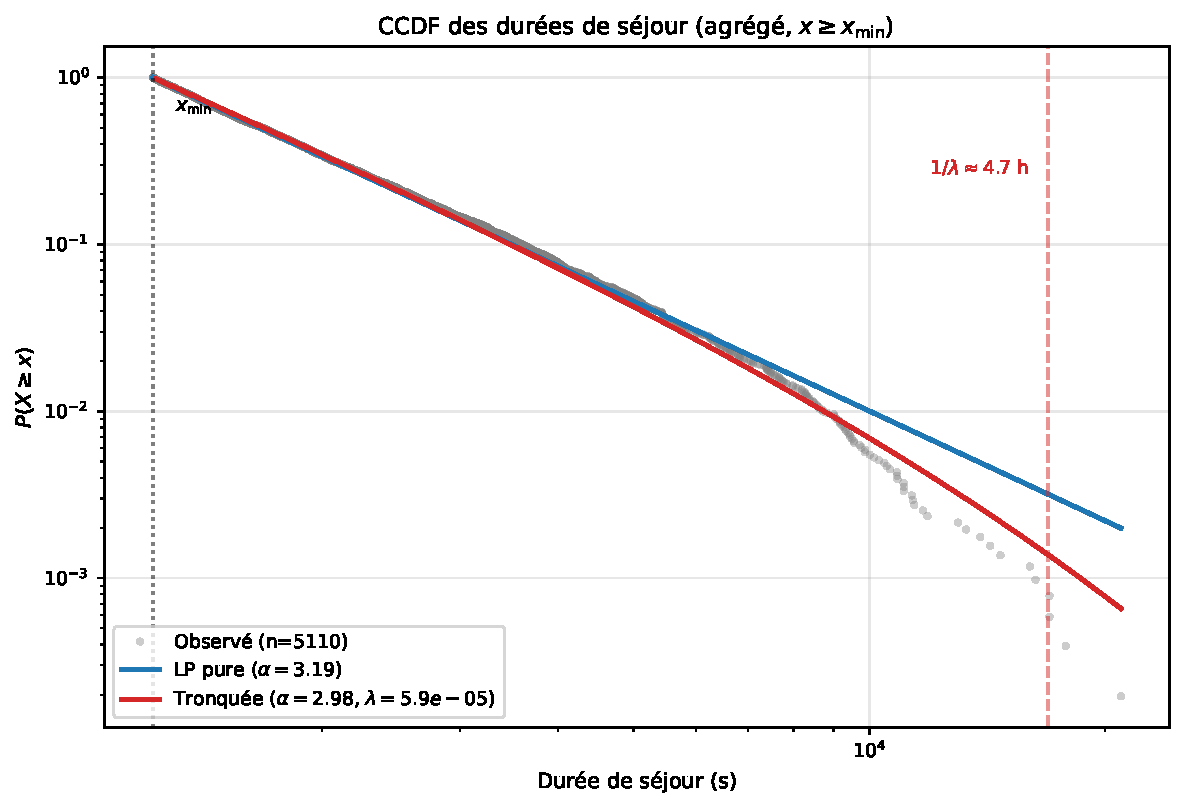
\includegraphics[width=0.85\linewidth]{graphe_9_ccdf_sejour.pdf}
\caption{Fonction de survie empirique des durées de séjour non censurées
($n = 5\,110$ au-dessus de $x_{\min}$), avec les ajustements de la loi de puissance
pure ($\alpha = 3{,}19$) et de la loi tronquée ($\alpha = 2{,}98$,
$\lambda = 5{,}9 \times 10^{-5}$~s$^{-1}$). La ligne verticale rouge marque
$1/\lambda \approx 4{,}7$~h. La tronquée suit mieux que la loi pure entre
$x_{\min}$ et $2 \times 10^4$~s, mais les deux modèles surestiment la queue
au-delà.}
\label{fig:lp-ccdf-sejour}
\end{figure}

Le $\hat\alpha = 3{,}19$ est au-dessus de la fourchette 1{,}5--2{,}5 usuellement rapportée
pour les temps de séjour~\cite{gonzalez2008,alessandretti2017}. Ceci suggère soit un effet
de bord (le filtre non-censuré coupe la queue), soit un effet du filtre
\code{MIN_POINTS = 300} appliqué en amont, soit une différence de définition des arrêts.
La valeur n'est pas aberrante en soi, mais elle mérite discussion.

\subsection{Distance à l'intérieur d'un même segment (\code{distance})}

Sur 1\,283 paires, l'exposant est $\hat\alpha = 2{,}026$, $p_{\text{boot}} = 0{,}055$ :
verdict \emph{rejetée}, mais le meilleur modèle AICc reste la loi de puissance (poids
0{,}528), et aucune alternative ne la bat significativement. C'est un cas
\textbf{ambigu} : le test d'adéquation rejette, mais la comparaison AICc ne lui préfère
pas clairement une autre loi. Le verdict a été consolidé avec $B = 1000$ (contre $B = 500$
dans une version antérieure) : le rejet est confirmé, et même renforcé ($p$ passe de
$0{,}070$ à $0{,}055$). Sur la figure~\ref{fig:lp-ccdf-autres}, les points de queue
restent au-dessus des courbes, ce qui traduit une queue plus lourde que celle des deux
modèles ajustés.

\subsection{Séjours incluant les censurés (\code{sejour_avec_censurees})}

Sur 13\,378 séjours (censurés inclus), $\hat\alpha = 2{,}365$, $p_{\text{boot}} < 0{,}001$ :
rejetée. Le $\hat{x}_{\min}$ de cet ajustement est \textbf{29\,918~s (environ 9~heures)},
ce qui signifie que la loi de puissance ne s'ajuste que sur les pauses de plus de 9~h.
Ceci n'est pas surprenant : cette variable inclut les \emph{pauses entre segments}, dont
la durée est celle du trou d'enregistrement (appareil éteint). La distribution est donc
\emph{bimodale} : une population de vrais séjours (courts, pendant l'enregistrement) et
une population d'absences (longues, pendant l'extinction). L'ajustement trouve le
$x_{\min}$ dans la zone des absences, ce qui produit un $\hat\alpha$ formellement correct
mais physiquement non interprétable. Sur la figure~\ref{fig:lp-ccdf-autres}, la queue est
approximativement en loi de puissance sur deux décades, mais la taille de l'échantillon
permet de rejeter l'ajustement. \textbf{Cette variable doit être considérée comme une
variable de sensibilité, non comme un résultat principal.}

\subsection{Distance à cheval (\code{distance_a_cheval})}

Sur 10\,216 paires (incluant les sauts à travers un trou), $\hat\alpha = 1{,}779$,
$p_{\text{boot}} < 0{,}001$ : rejetée. La loi de puissance tronquée obtient le meilleur
poids AICc (0{,}511), avec un avantage marginal ($p_{\text{Vuong}} = 0{,}099$). Le
$\hat\alpha = 1{,}78$ est dans la fourchette publiée pour les distances
inter-arrêts~\cite{rhee2011,alessandretti2017}. Le paramètre ajusté
$\lambda = 6{,}58 \times 10^{-9}$~m$^{-1}$ correspond à une échelle
$1/\lambda \approx 1{,}5 \times 10^5$~km, très au-delà des distances observées
($\le 50$~km). La tronquée « gagne » donc sur des queues extrêmes peuplées par les sauts
à travers trou, mais reste essentiellement une loi de puissance sur le domaine utile.
Contrairement au cas \texttt{sejour}, la coupure n'est pas physiquement interprétable.
Sur la figure~\ref{fig:lp-ccdf-autres}, un plateau entre $10^5$ et $2 \times 10^6$~m, où
les données sont environ trois fois au-dessus des courbes, précède une coupure brutale
vers $10^7$~m. Le test d'adéquation de la tronquée donne $p=1{,}000$, ce qui peut sembler
un excellent résultat. C'est un artefact : avec $\lambda \to 0$, la tronquée est
numériquement équivalente à la loi de puissance, elle-même rejetée par le test de Clauset
($p<0{,}001$). Le $p=1{,}000$ ne fait que refléter que, à cette résolution et avec
$x_{\min}$ fixé, les données ne s'écartent pas de manière détectable d'une loi de
puissance pure — ce que le test de Clauset contredit. \textbf{Aucune loi du catalogue
n'est adéquate pour cette variable.}

\begin{figure}[ht]
\centering
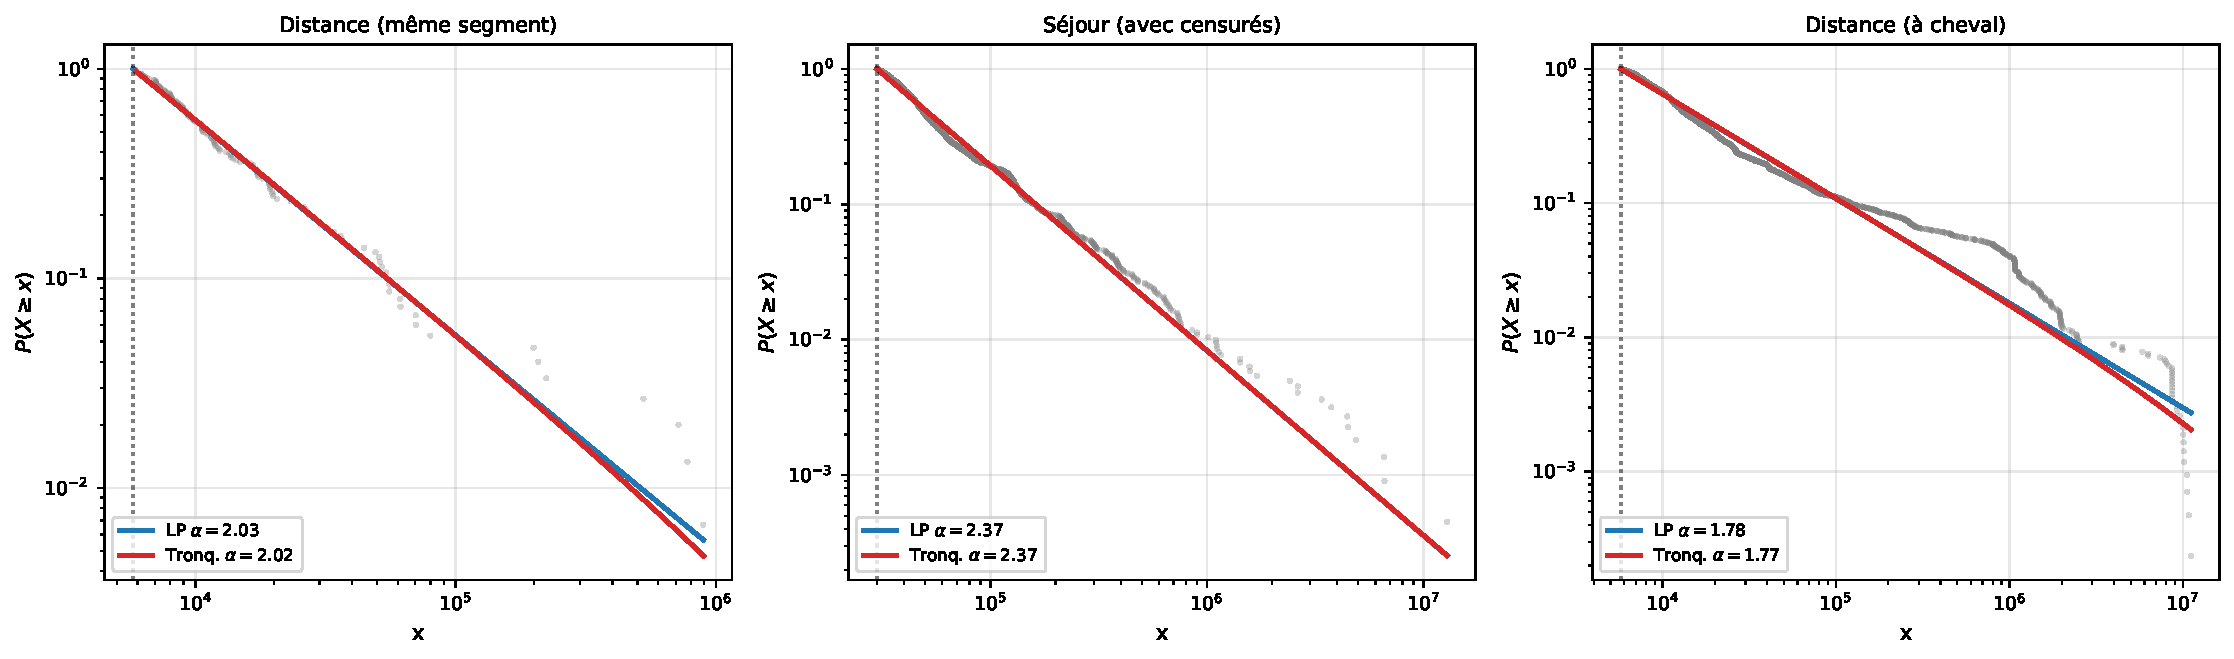
\includegraphics[width=\linewidth]{graphe_13_ccdf_autres.pdf}
\caption{Fonctions de survie empiriques des trois autres variables, avec les
ajustements de la loi de puissance pure (bleu) et de la loi tronquée (rouge).
\emph{Gauche} : distance à l'intérieur d'un même segment (m) — les points de queue
sont au-dessus des courbes (queue plus lourde que les modèles), l'ajustement est
raisonnable jusqu'à $10^5$~m. \emph{Centre} : séjour avec censurés (s) — la queue
est approximativement en loi de puissance sur deux décades, mais la taille de
l'échantillon ($n = 13\,378$) permet de rejeter l'ajustement. \emph{Droite} :
distance à cheval (m) — plateau entre $10^5$ et $2 \times 10^6$~m où les données
sont environ trois fois au-dessus des courbes, puis coupure vers $10^7$~m (échelle
terrestre).}
\label{fig:lp-ccdf-autres}
\end{figure}

\section{Sensibilité aux seuils d'arrêt}
\label{sec:lp-sensibilite}

Les résultats agrégés de la section~\ref{ch:lp-resultats} utilisent le jeu de
seuils d'arrêt par défaut ($R_{\mathrm{arr}} = 200$~m, $T_{\min} = 1200$~s).
Comme pour la segmentation temporelle (section~\ref{ch:prep}), ce choix est un
arbitrage et non une prescription de la littérature. Nous l'avons donc fait
varier sur les quatre couples de \code{ARRET_JEUX_SENSIBILITE} :
$(100, 300)$, $(100, 600)$, $(200, 1200)$, $(200, 1800)$.

\begin{table}[ht]
\centering
\caption{Sensibilité de $\alpha$ aux quatre jeux de seuils d'arrêt (population
agrégée, $B = 50$ ; les $\sigma_\alpha$ sont de l'ordre de 0{,}02--0{,}05).}
\label{tab:lp-sensibilite}
\small
\begin{tabular}{lrrrr}
\toprule
Jeu & $n_{\text{séjour}}$ & $\alpha_{\text{séjour}}$ & $n_{\text{distance}}$ & $\alpha_{\text{distance}}$ \\
\midrule
100~m~/~5~min  & 32\,110 & 3{,}12 & 13\,806 & 1{,}89 \\
100~m~/~10~min & 14\,185 & 3{,}18 & 4\,064  & 1{,}82 \\
200~m~/~20~min & 5\,354  & 3{,}19 & 1\,283  & 2{,}03 \\
200~m~/~30~min & 2\,789  & 3{,}42 & 428    & 1{,}54 \\
\bottomrule
\end{tabular}
\end{table}

\begin{figure}[ht]
\centering
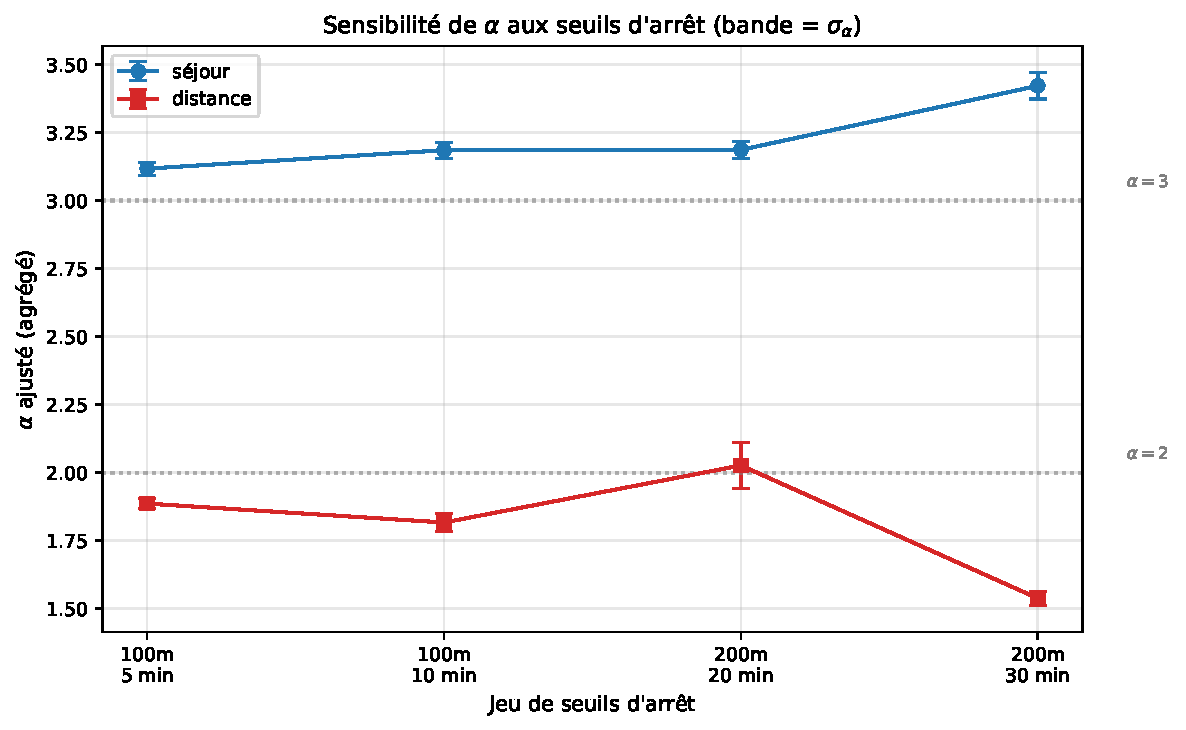
\includegraphics[width=0.85\linewidth]{graphe_12_sensibilite.pdf}
\caption{Sensibilité de l'exposant $\alpha$ aux quatre jeux de seuils d'arrêt
(population agrégée, barres d'erreur = $\sigma_\alpha$). L'exposant des séjours
reste au-dessus de 3 aux quatre jeux, donc hors du domaine $]2, 3[$ de la relation
ON/OFF. L'exposant des distances (même segment) varie de 1{,}54 à 2{,}03 ; la
valeur basse du jeu 200~m~/~30~min repose sur $n = 428$ seulement et reflète la
taille de l'échantillon plutôt qu'une propriété de la distribution.}
\label{fig:lp-sensibilite}
\end{figure}

La figure~\ref{fig:lp-sensibilite} montre deux comportements distincts.
L'exposant des séjours est \emph{monotone croissant} avec la durée minimale
d'arrêt (3{,}12 à 3{,}42) : un seuil plus exigeant élimine les séjours courts et
durcit la queue. L'amplitude reste modérée ($\Delta \alpha = 0{,}30$), et surtout
\textbf{$\alpha_{\text{séjour}}$ reste au-dessus de 3 aux quatre jeux}, donc
toujours hors du domaine $]2, 3[$ où la relation ON/OFF $H = (4 - \alpha)/2$
s'applique. \textbf{Le résultat « $\alpha_{\text{séjour}}$ hors domaine » est
robuste au choix de seuils}, ce qui est un argument fort en faveur de la
conclusion négative sur le lien ON/OFF.

L'exposant des distances est plus variable (1{,}54 à 2{,}03). La chute à 1{,}54
pour le jeu 200~m~/~30~min est un artefact : avec $n = 428$ paires seulement, la
queue de l'échantillon est instable. Sur les trois jeux les mieux pourvus en
données, $\alpha_{\text{distance}} \in [1{,}82, 2{,}03]$, compatible avec la
fourchette publiée pour les distances inter-arrêts.

\begin{limite}
Le jeu de seuils par défaut (200~m~/~20~min) donne $\alpha_{\text{séjour}} = 3{,}19$,
proche du minimum des quatre valeurs testées. Ce n'est pas un choix biaisé en
faveur d'une conclusion, mais il faut noter que toute valeur d'$\alpha$ citée dans
ce chapitre doit être accompagnée de son jeu de seuils. Sur les quatre jeux,
cependant, la conclusion qualitative (loi de puissance pure rejetée pour les
séjours) ne change pas.
\end{limite}

\section{Discussion : \code{distance} vs \code{distance_a_cheval}}

La figure~\ref{fig:lp-ccdf-autres} montre les trois autres variables ; seule la
distance à l'intérieur d'un même segment présente une queue qui reste au-dessus des
ajustements, ce qui complique l'interprétation de $\alpha = 2{,}03$.

Le choix de la variable « distance » est un arbitrage entre pureté et volume :

\begin{itemize}
\item \code{distance} (même segment) : \textbf{1\,283 paires}, aucune traversée de trou,
mais 90~\% des paires éliminées (car les arrêts consécutifs sont presque toujours dans
des segments différents).
\item \code{distance_a_cheval} : \textbf{10\,216 paires}, mais certaines traversent un
trou d'enregistrement. Des arrêts intermédiaires ont pu passer inaperçus, ce qui gonfle
les distances et abaisse mécaniquement $\hat\alpha$.
\end{itemize}

\begin{choix}[Deux variables, deux résultats]
Nous rapportons les deux, en les interprétant comme des bornes. \code{distance} donne
$\hat\alpha = 2{,}03$ (proche de la borne basse de la littérature), \code{distance_a_cheval}
donne $\hat\alpha = 1{,}78$ (dans la fourchette). La vérité est probablement entre les
deux, et le biais de chaque variante est documenté. Un ajustement plus fin (retirer les
paires traversant un trou de plus de 15~min) reste à faire.
\end{choix}

\section{Conséquence pour le lien ON/OFF}

La relation $H = (4-\alpha)/2$ ne s'applique que pour $2 < \alpha < 3$. Le tableau
suivant applique cette contrainte aux quatre résultats :

\begin{table}[ht]
\centering
\caption{Application de la relation ON/OFF aux quatre résultats.}
\label{tab:onoff-applique}
\small
\begin{tabular}{lrrll}
\toprule
Variable & $\alpha$ & Dans domaine ? & $H_{\text{pred}}$ & Fiabilité \\
\midrule
\code{sejour} & $3{,}19$ & non ($\alpha > 3$) & --- & --- \\
\code{distance} (même seg.) & $2{,}03$ & \textbf{oui} & $0{,}987$ & faible (verdict rejetée, $p=0{,}055$) \\
\code{sejour_avec_censurees} & $2{,}37$ & \textbf{oui} & $0{,}817$ & très faible (bimodale probable) \\
\code{distance_a_cheval} & $1{,}78$ & non ($\alpha < 2$) & --- & --- \\
\bottomrule
\end{tabular}
\end{table}

\paragraph{Conclusion.} \textbf{Aucun $H_{\text{pred}}$ calculable n'est solide.}
\begin{itemize}
\item Pour \code{distance} (même seg.), $H_{\text{pred}} \approx 0{,}99$ est proche de 1
(marche aléatoire), valeur atypique pour la mobilité, et le verdict est rejeté.
\item Pour \code{sejour_avec_censurees}, $H_{\text{pred}} \approx 0{,}82$ est cohérent
avec le 0{,}726 mesuré par DFA, mais la variable est probablement bimodale, donc non
interprétable.
\end{itemize}
\textbf{Aucune conclusion ne peut être tirée à ce stade sur la cohérence du lien ON/OFF
sur données réelles.} L'écart apparent entre $H_{\text{pred}} = 0{,}82$ et
$H_{\text{DFA}} = 0{,}726$ \emph{pourrait} être cohérent avec la prédiction (avec une
marge d'incertitude), mais l'hypothèse bimodale interdit de le présenter comme une
confirmation.

\section{Limites spécifiques à cette analyse}

\begin{limite}[La victoire de la tronquée n'est pas toujours physique]
Le paramètre de coupure $\lambda$ est maintenant exporté et interprété. Pour
\texttt{sejour}, $\lambda$ correspond à une coupure à $\approx 4{,}7$~h, compatible avec
la périodicité circadienne. Pour \texttt{distance\_a\_cheval}, $\lambda$ est négligeable
sur le domaine observé ($1/\lambda \approx 1{,}5 \times 10^5$~km) : la tronquée gagne par
flexibilité statistique sur les queues extrêmes, pas par coupure réelle. Le cas
\texttt{sejour\_avec\_censurees} a $\lambda \approx 10^{-17}$, numériquement nul : la
tronquée y est identique à la loi de puissance pure.
\end{limite}

\begin{limite}[Test d'adéquation de la tronquée : puissance limitée]
Le test bootstrap d'adéquation de la tronquée (tableau~\ref{tab:lp-adequation})
diffère du test de Clauset sur deux points : (i) $x_{\min}$ est fixé à sa valeur
observée au lieu d'être re-choisi à chaque simulation, ce qui divise le coût par
$\sim 3$ mais retire la sensibilité à un mauvais choix de seuil ; (ii) seuls
$\alpha$ et $\lambda$ sont réajustés sur chaque simulation. Conséquence : le test
est \emph{beaucoup moins puissant} que le test de Clauset. Un $p > 0{,}1$ sur ce
test ne prouve \emph{pas} que la tronquée est adéquate ; il indique seulement que
les données ne s'en écartent pas de manière détectable à cette résolution. Un
$p \le 0{,}1$, en revanche, est un rejet robuste (le test est permissif, donc s'il
rejette, c'est que le désaccord est net) : c'est le cas de \texttt{sejour} à
$p<0{,}005$. Une implémentation plus rigoureuse (re-choix de $x_{\min}$ à chaque
simulation) donnerait un test plus puissant mais coûterait $\sim 3\times$ plus
cher ; elle n'a pas été retenue ici.
\end{limite}

\begin{limite}[Un seul jeu de données exploitable]
L'analyse des lois de puissance n'a été possible que sur GeoLife. T-Drive, testé
en sensibilité (section~\ref{sec:tdrive}), ne produit pas de distribution
interprétable : les arrêts détectés sont dominés par le stationnement nocturne
pour les durées, et par des courses entières pour les distances. Aucune
comparaison inter-corpus n'a donc pu être menée.
\end{limite}

\begin{limite}[37 utilisateurs exclus]
Comme documenté au chapitre~\ref{ch:prep}, \code{MIN_POINTS = 300} exclut 37
utilisateurs sur 183. Leur contribution potentielle à la distribution des durées de
séjour et des distances n'est pas connue. Une analyse de sensibilité avec
\code{MIN_POINTS = 50} permettrait de quantifier ce biais.
\end{limite}

\begin{limite}[Typologie impossible avec 15 utilisateurs]
Avec \code{LP_NB_MIN_PAR_UTILISATEUR = 100}, seuls 15 utilisateurs sur 137 ont assez
de séjours pour une analyse individuelle. C'est \textbf{insuffisant} pour l'ACP et le
K-means prévus dans la tâche 2.3.5 du mémoire. Trois options sont possibles : abaisser le
seuil à 50, utiliser \code{distance_a_cheval} (plus d'observations par user), ou
renoncer à la typologie quantitative. Décision à discuter avec l'encadrant.
\end{limite}

\section{Synthèse}

\begin{table}[ht]
\centering
\caption{Synthèse des résultats lois de puissance sur GeoLife.}
\label{tab:lp-synthese}
\small
\begin{tabular}{lr}
\toprule
Indicateur & Valeur \\
\midrule
Utilisateurs analysés (au moins un arrêt) & 137 \\
Jeu de seuils d'arrêt & 200~m~/~20~min \\
Loi de puissance pure gagnante & aucune \\
Loi de puissance tronquée gagnante & \code{sejour}, \code{distance_a_cheval} \\
Loi de puissance tronquée adéquate (bootstrap) & aucune \\
Cas ambigu & \code{distance} (même seg.) \\
Cas ininterprétable (bimodale) & \code{sejour_avec_censurees} \\
$\alpha$ dans $[2,3]$ (domaine ON/OFF) & 2 variables \\
$H_{\text{pred}}$ solide & aucun \\
\bottomrule
\end{tabular}
\end{table}

\paragraph{Message à retenir.} La loi de puissance pure n'est pas confirmée sur ce
corpus. La loi de puissance tronquée obtient le meilleur AICc sur deux des quatre
variables, mais elle est rejetée par le test bootstrap sur la variable la plus importante
(\texttt{sejour}). Aucune des cinq lois du catalogue n'est donc adéquate pour les durées
de séjour. Le résultat honnête est double : la queue des séjours présente une coupure
cohérente avec la périodicité circadienne (information positive sur le processus), mais
aucun modèle paramétrique simple ne la décrit (résultat négatif sur la modélisation). La
discussion vers une coupure exponentielle reste pertinente, mais elle doit être présentée
comme une piste, pas comme un résultat acquis. Aucune prédiction ON/OFF solide ne peut
être tirée.

% =====================================================================
\chapter{Extension proposée : segmentation par labels de transport}
\label{ch:labels}
% =====================================================================

\emph{Ce chapitre décrit une extension \textbf{proposée} ; elle n'est pas implémentée.}

\section{Motivation}

Un segment qui mélange plusieurs modes de transport est un changement de régime de vitesse,
que la littérature montre facile à confondre avec de la mémoire
longue~\cite{diebold2001}. Les labels apportent des segments mono-mode, une stratification
par mode, et une vérité terrain partielle pour la détection de régimes.

\section{Procédure proposée}

\begin{enumerate}
  \item lire \code{labels.txt} (début, fin, mode) et convertir en secondes UNIX UTC ;
  \item attribuer à chaque point le mode de l'intervalle qui le contient, \emph{non
  étiqueté} sinon ;
  \item regrouper les labels en classes (marche, vélo, véhicule routier, bus, rail, avion,
  bateau) ;
  \item couper aux changements de classe, sans raccorder ;
  \item appliquer les filtres de longueur habituels.
\end{enumerate}

\section{Usages scientifiques}

\begin{itemize}
  \item $\hat H$ par mode mono-mode, isolant l'effet du mélange de régimes ;
  \item vérité terrain pour le détecteur MAD (taux de détection et de fausses alarmes) ;
  \item garde-fou par mode : quantiles des vitesses par classe pour remplacer le seuil
  unique de 200~km/h.
\end{itemize}

\section{Limites attendues}

Couverture partielle (69 utilisateurs), qualité incertaine des labels (saisis manuellement),
fragmentation des segments après coupure, circularité potentielle si les mêmes labels
servent à couper et à évaluer.

% =====================================================================
\chapter{Résultats sur GeoLife (Hurst)}
\label{ch:exp}
% =====================================================================

\section{Configuration de référence et chiffres agrégés}

Tous les chiffres de ce chapitre sont produits avec \code{TIME_GAP_THRESHOLD = 900},
\code{MIN_POINTS = 300}, sur les 145 utilisateurs de GeoLife ayant au moins un segment
retenu. L'empreinte de configuration de cette exécution est reportée dans le
tableau~\ref{tab:corpus}.

\section{Distribution des $\hat H$ : tous vs gardés}

\begin{table}[ht]
\centering
\caption{Moyennes de $\hat H$ par méthode, tous segments et segments gardés.}
\label{tab:moyennes-H}
\small
\begin{tabular}{lrrr}
\toprule
Population & $\hat H_{\mathrm{DFA}}$ & $\hat H_{\mathrm{RS}}$ & $\hat H_{\mathrm{Whittle}}$ \\
\midrule
Tous segments (145 users) & 0{,}834 & 0{,}776 & 0{,}802 \\
Segments gardés (136 users) & \textbf{0{,}726} & \textbf{0{,}723} & \textbf{0{,}728} \\
Segments gardés, pondéré par $n_{\text{gardés}}$ & 0{,}741 & 0{,}731 & 0{,}740 \\
\bottomrule
\end{tabular}
\end{table}

\begin{figure}[ht]
\centering
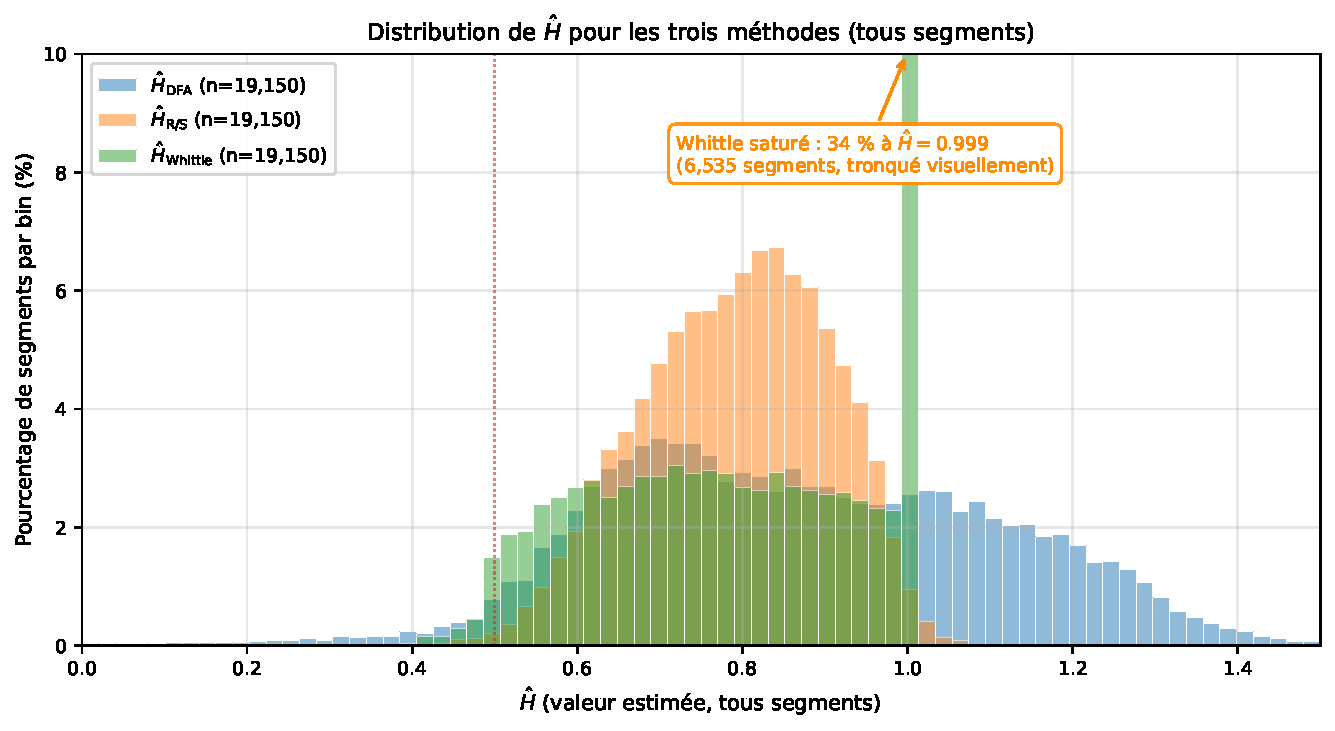
\includegraphics[width=\textwidth]{graphe_2_distribution.pdf}
\caption{Distribution de $\hat H$ sur les 19\,150 segments retenus (gris) et les
7\,853 segments gardés (bleu), pour les trois méthodes. Le filtre élimine la queue
super-diffusive ($\hat H > 1$), la saturation Whittle ($\hat H = 1$, $n = 5\,365$)
et déplace la médiane de $0{,}857$ à $0{,}736$ (DFA). Ce déplacement n'est pas une
amélioration de la précision : c'est un changement de population.}
\label{fig:distribution}
\end{figure}

\paragraph{Lecture.} Le filtre agit surtout sur DFA (baisse de $0{,}11$ en moyenne,
$0{,}12$ en médiane ; visible sur la figure~\ref{fig:distribution}) : c'est la
méthode la plus sensible à la non-stationnarité. R/S baisse de $0{,}05$, Whittle de
$0{,}08$. L'écart entre la moyenne arithmétique (par utilisateur) et la moyenne pondérée
(par segment) reflète la concentration des segments gardés : les cinq plus gros
utilisateurs portent 25,4~\% des segments gardés, et leurs H sont supérieurs à la moyenne.

\section{Concentration et dispersion}

\begin{table}[ht]
\centering
\caption{Dispersion de $\hat H_{\mathrm{DFA}}$ sur les segments gardés, par strate d'effectif.}
\label{tab:dispersion}
\small
\begin{tabular}{lrr}
\toprule
Strate & Nombre d'utilisateurs & $\hat H_{\mathrm{DFA, gardés}}$ (moy $\pm$ écart-type) \\
\midrule
$n_{\text{gardés}} \ge 50$ & 43 & $0{,}738 \pm 0{,}038$ \\
$n_{\text{gardés}} < 10$ & 45 & $0{,}712 \pm 0{,}096$ \\
\bottomrule
\end{tabular}
\end{table}

\begin{figure}[ht]
\centering
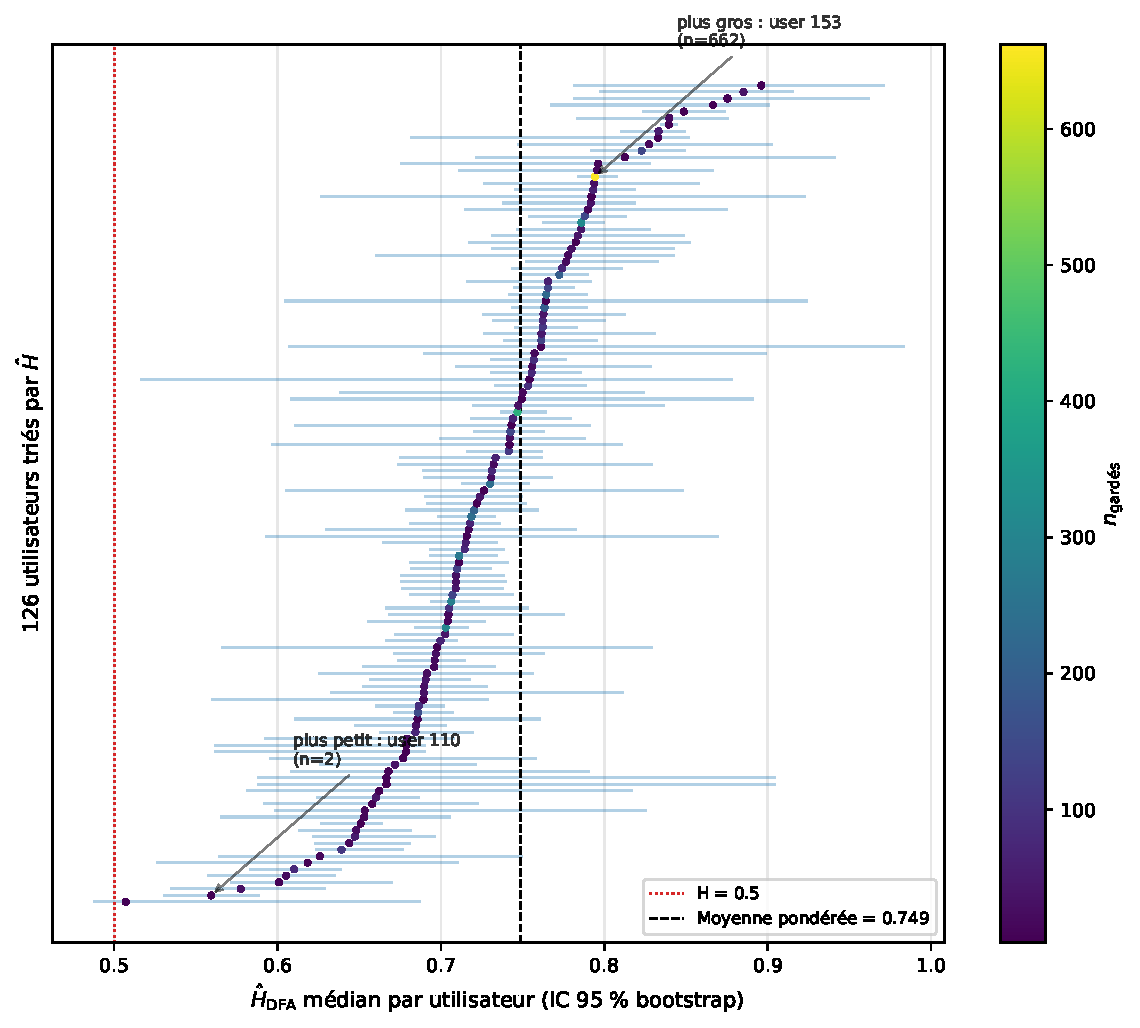
\includegraphics[width=0.8\textwidth]{graphe_4_user_ic.pdf}
\caption{$\hat H_{\mathrm{DFA}}$ médian par utilisateur (126 utilisateurs avec au moins
2 segments gardés), trié par valeur croissante, avec intervalle de confiance à 95\,\%
obtenu par bootstrap sur les segments ($B = 1\,000$). La couleur encode le nombre de
segments gardés. La largeur des intervalles décroît avec $n_{\text{gardés}}$ : la
dispersion inter-utilisateurs est en grande partie du bruit d'échantillonnage.}
\label{fig:user_ic}
\end{figure}

La dispersion observée est compatible avec un bruit d'échantillonnage dominant (les
utilisateurs à faible effectif ont une variance plus grande), sans exclure une
hétérogénéité réelle résiduelle. La figure~\ref{fig:user_ic} rend visible ce point :
les utilisateurs à faible effectif (couleur foncée) ont des intervalles qui se
recouvrent, rendant l'ordre non significatif.

\section{Neuf utilisateurs sans segment gardé}

Neuf utilisateurs (049, 056, 079, 114, 120, 137, 151, 157, 166) n'ont aucun segment gardé.
Six d'entre eux ont $\hat H_{\mathrm{DFA}} > 1$ sur la totalité des segments : leur
trajectoire est super-diffusive sur l'ensemble du fichier. Trois cas sont marginaux :
151 et 157 (1 segment chacun, $\hat H_{\mathrm{DFA}} < 1$) et 120 (5 segments,
$\hat H_{\mathrm{DFA}} = 0{,}90$). Ces utilisateurs ne peuvent pas recevoir de valeur de
$H$ dans le cadre du filtre strict ; ils peuvent représenter un régime balistique légitime,
non du bruit.

\section{Doublons détectés}

Trois paires d'utilisateurs ont des lignes strictement identiques dans la synthèse :
$055/075$, $058/059$, $069/129$ ; et une paire partage le même $H_{\text{gardés}}$ avec des
totaux différents : $046/121$. L'origine (fichiers source dupliqués ou problème en amont
dans \code{resultats_H/}) n'a pas été identifiée. Ces doublons représentent 39 segments
gardés (0,50~\%), numériquement négligeable, mais doivent être documentés avant toute
agrégation inter-utilisateurs.

\section{Synthèse}

\begin{table}[ht]
\centering
\caption{Synthèse des estimations sur GeoLife (config \code{TIME_GAP}=900).}
\label{tab:synthese}
\small
\begin{tabular}{lr}
\toprule
Indicateur & Valeur \\
\midrule
Segments retenus & 19\,150 \\
Segments gardés & 7\,853 (41,0~\%) \\
Utilisateurs avec au moins un gardé & 136 \\
$\hat H_{\mathrm{DFA}}$ (moyenne par user) & 0{,}726 \\
$\hat H_{\mathrm{DFA}}$ (pondéré par $n_{\text{gardés}}$) & 0{,}741 \\
Convergence DFA~$/$~Whittle sur les gardés & $\pm 0{,}02$ \\
Biais R/S corrigé à $H \ge 0{,}7$ (mesuré sur fGn) & $-0{,}15$ \\
\bottomrule
\end{tabular}
\end{table}

\paragraph{Ce qu'il faut retenir.} La valeur $\hat H_{\mathrm{DFA}} \approx 0{,}726$ sur
GeoLife \emph{n'est pas} une estimation de la mémoire longue du déplacement. Elle mesure
ce que DFA produit sur la série $d_i$ filtrée. Le test décisif (à $\rho_1$ contrôlé) a
montré que DFA \emph{peut} distinguer fGn et AR(1) à même $\rho_1$, mais avec un écart
$\sim 0{,}07$, du même ordre que le RMSE d'estimation. La séparation est statistique (sur
19\,150 segments), pas pratique (par segment).

% =====================================================================
\chapter{Discussion et perspectives}
\label{ch:discussion}
% =====================================================================

\section{Ce que le travail permet et ne permet pas}

Le pipeline produit, pour chaque segment, une estimation de $H$ accompagnée de drapeaux
qui disent dans quelle mesure elle est interprétable, et une précision de référence mesurée
par simulation. Il ne permet pas, à lui seul, de conclure à une mémoire longue : un
dépassement du modèle nul ne distingue pas mémoire longue et alternance de régimes, et un
exposant supérieur à 1 n'est pas une estimation de $H$.

\section{Limites d'ensemble}

\begin{itemize}
  \item \textbf{Circularité du filtre.} Le filtre de fiabilité (section~\ref{sec:circularite})
  conditionne l'estimation sur $H$ lui-même. Le $\hat H_{\text{gardés}}$ est conditionnel,
  pas populationnel.
  \item \textbf{Validité de construit.} La série des $d_i$ mélange vitesse et intervalle de
  temps ; une valeur de $H$ est avant tout une propriété de la \emph{série} et du
  prétraitement, pas nécessairement de la mobilité.
  \item \textbf{Mémoire longue ou régimes.} Le test de dépassement ne les distingue
  pas~\cite{diebold2001}.
  \item \textbf{Non-stationnarité.} \code{statio_p_value} est inférieure à $10^{-20}$ sur
  la quasi-totalité des segments gardés. Le $H_{\text{gardés}}$ est un $H$ effectif, non
  un $H$ de processus stationnaire.
  \item \textbf{Estimateurs.} DFA sensible aux tendances ; R/S corrigé biaisé à haute
  persistance (mesuré) ; Whittle local limité à $H<1$ et collé à la borne en cas de
  non-stationnarité.
  \item \textbf{Un seul dataset exploitable.} T-Drive est incompatible avec l'estimation
  de $H$ sur $d_i$ (section~\ref{sec:tdrive}) et avec l'analyse des lois de puissance
  (les arrêts détectés correspondent au stationnement nocturne des taxis, pas à des
  pauses fonctionnelles). Aucune analyse n'a donc pu être répliquée sur un second corpus.
  \item \textbf{Constantes.} De nombreuses constantes sont des planchers absolus derrière
  des seuils relatifs (annexe~\ref{app:params}).
  \item \textbf{Lois de puissance.} La loi de puissance pure n'est jamais le meilleur
  modèle AICc ; la tronquée gagne sur deux variables mais est rejetée par le test
  bootstrap sur la plus importante (\texttt{sejour}) ; aucune des cinq lois n'est adéquate
  pour les séjours. Le cas \code{distance} est ambigu ($p=0{,}055$, juste sous le seuil).
  \item \textbf{Test d'adéquation tronquée permissif.} Le test bootstrap de la tronquée
  (section~\ref{ch:lp-resultats}) fixe $x_{\min}$ à sa valeur observée au lieu de le
  re-choisir à chaque simulation, ce qui le rend beaucoup moins puissant que le test de
  Clauset. Un $p > 0{,}1$ sur ce test ne prouve pas que la tronquée est adéquate ; il
  indique seulement qu'à cette résolution, les données ne s'en écartent pas de manière
  détectable.
  \item \textbf{Biais de sélection LP.} 37 utilisateurs exclus par \code{MIN_POINTS=300}
  sans justification pour les lois de puissance.
  \item \textbf{Typologie impossible.} 15 utilisateurs avec $\ge 100$ séjours : trop peu
  pour ACP+K-means.
\end{itemize}

\section{Perspectives}

\begin{enumerate}
  \item \textbf{Test fGn du filtre.} Passer des fGn de $H_0$ connu dans le filtre de
  fiabilité et mesurer le biais induit par la sélection. C'est le test le plus critique
  pour interpréter le 0{,}726.
  \item \textbf{Agrégation de \code{nul_p}.} Quantifier la fraction de segments gardés
  qui rejettent le modèle nul AR(p), à $p=1$ et $p=5$.
  \item \textbf{Bootstrap par utilisateur.} Estimer l'incertitude sur le H global en
  rééchantillonnant les utilisateurs, pas les segments.
  \item \textbf{Série à pas régulier.} Ré-échantillonner chaque segment à pas fixe pour
  répondre à la question de la dépendance en temps physique.
  \item \textbf{Whittle local exact} (Shimotsu--Phillips) et bande passante variable.
  \item \textbf{Test multi-estimateurs} du modèle nul, avec correction pour tests multiples.
  \item \textbf{Deux branches de traitement} : segments continus pour $H$ ; chronologie par
  utilisateur pour les séjours.
  \item \textbf{Fusion des arrêts proches} et vraisemblance avec censure.
  \item \textbf{Segmentation par labels} et coupure aux changements de régime.
  \item \textbf{Analyse de sensibilité \code{MIN_POINTS=50} pour les LP.}
  Régénérer \code{sortie/} avec un seuil plus bas, relancer l'analyse LP sur l'ensemble
  élargi, comparer les $\alpha$ agrégés. Quantifie le biais de sélection.
  \item \textbf{Vérifier la bimodalité de \code{sejour_avec_censurees}.} Histogramme
  log-log des durées ; confirmer ou infirmer l'hypothèse (30 secondes de code).
  \item \textbf{Consolider $p_{\text{boot}}$ pour \code{distance}.} Relancer avec
  $B = 1000$ : le verdict est confirmé à 0{,}055, la consolidation est faite.
  \item \textbf{Décider d'une stratégie typologie.} Baisser \code{LP_NB_MIN_PAR_UTILISATEUR}
  à 50, utiliser \code{distance_a_cheval}, ou abandonner la typologie quantitative.
  \item \textbf{Typologie et cartographie} (ACP, K-means), puis extension à d'autres jeux
  de données.
\end{enumerate}

% =====================================================================
\chapter*{Conclusion}
\addcontentsline{toc}{chapter}{Conclusion}
% =====================================================================

Ce mémoire a présenté une chaîne complète, du fichier GPS brut à l'ajustement de lois de
puissance, avec pour principe de ne jamais cacher ce qui limite l'interprétation : points
suspects marqués plutôt que supprimés, durées censurées étiquetées, estimations hors
domaine signalées, test de dépassement dont on mesure les faux positifs, filtre de
fiabilité dont on explicite la circularité.

Sur le volet Hurst, les résultats obtenus (19\,150 segments retenus, 7\,853 gardés,
$\hat H_{\mathrm{DFA}} \approx 0{,}726$ sur les gardés) ne démontrent pas la mémoire longue
du déplacement humain. Ils quantifient une persistance locale dont la robustesse aux
régimes et au bruit d'échantillonnage n'est pas établie. La question de la mémoire longue
reste ouverte, et sa résolution nécessite une série d'un autre type (événements, agrégats
spatio-temporels) que celle utilisée ici.

Sur le volet lois de puissance, l'analyse sur 137 utilisateurs donne un résultat négatif
partiel mais solide : la loi de puissance pure n'est jamais le meilleur modèle AICc, et la
\emph{loi de puissance tronquée} l'emporte sur deux variables (\code{sejour} et
\code{distance_a_cheval}), avec des poids AICc de 0{,}97 et 0{,}51. Mais cette victoire
AICc ne suffit pas : un test bootstrap d'adéquation rejette la tronquée sur
\texttt{sejour} ($p<0{,}005$), et son $p=1{,}000$ sur \texttt{distance\_a\_cheval} est un
artefact d'un $\lambda$ numériquement nul. \textbf{Aucune des cinq lois du catalogue n'est
adéquate pour les durées de séjour.} Le cas \code{distance} (même segment) reste ambigu
($p=0{,}055$), et \code{sejour_avec_censurees} est probablement bimodale. La relation
ON/OFF $H=(4-\alpha)/2$ ne peut être testée de façon fiable sur aucune variable : les deux
$\alpha$ dans le domaine $[2,3]$ reposent l'un sur un modèle rejeté, l'autre sur une
distribution bimodale.

La formulation à retenir est double :
\emph{« Sur des segments filtrés de GeoLife, le paramètre de Hurst estimé par DFA sur la
série des distances inter-points est d'environ $0{,}726$ ; ce chiffre ne peut pas être
interprété comme une mesure de la dépendance à longue portée du déplacement, mais il
quantifie une persistance locale dont la robustesse aux régimes et au bruit
d'échantillonnage n'est pas établie. »}
\emph{« Les distributions de durées de séjour et de distances inter-arrêts ne suivent pas
une loi de puissance pure. La loi de puissance tronquée est le meilleur des cinq modèles
testés pour les séjours, et sa coupure correspond à une échelle de $\approx 4{,}7$~h, mais
elle est rejetée par le test bootstrap : aucun modèle paramétrique simple n'est adéquat
pour les durées de séjour. La prédiction ON/OFF $H=(4-\alpha)/2$ ne peut pas être testée
de façon fiable sur ce corpus. »}

% =====================================================================
\appendix
\chapter{Paramètres du pipeline}
\label{app:params}
% =====================================================================

Les valeurs listées correspondent à \code{config.py} au moment de la rédaction
(configuration V5, \code{TIME_GAP_THRESHOLD = 900}). La colonne « Statut » distingue :
\textbf{conv.} (convention de la littérature), \textbf{emp.} (valeur empirique à
calibrer), \textbf{dév.} (interrupteur de développement), \textbf{num.} (paramètre
numérique).

{\small
\begin{longtable}{@{}p{4.9cm}p{1.8cm}p{5.9cm}p{1.0cm}@{}}
\caption{Constantes de \texttt{config.py} (V5, \texttt{TIME\_GAP=900}).}\label{tab:params}\\
\toprule
Constante & Valeur & Rôle & Statut \\
\midrule
\endfirsthead
\toprule
Constante & Valeur & Rôle & Statut \\
\midrule
\endhead
\bottomrule
\endfoot
\multicolumn{4}{@{}l}{\textit{Segmentation et sélection}}\\
\code{TIME_GAP_THRESHOLD} & 900 s & trou qui coupe un segment & emp.\\
\code{MIN_POINTS} & 300 & points minimaux d'un segment retenu & emp.\\
\code{MIN_POINTS_MORCEAU} & 50 & points minimaux d'un morceau (DFA) & emp.\\
\code{DISTANCE_MIN} & 0{,}1 km & distance minimale d'un segment retenu & emp.\\
\code{DISTANCE_MIN_RELATIF} & True & active le seuil relatif & emp.\\
\multicolumn{4}{@{}l}{\textit{Marquage}}\\
\code{MAX_SPEED} & 200 km/h & plancher absolu de vitesse & emp.\\
\code{MAX_SPEED_RELATIF} & 20 & multiple de la vitesse médiane & emp.\\
\code{MAX_DIST_M} & 30 & multiple de la distance médiane (mode relatif) & emp.\\
\code{MAX_DIST_M_ABSOLU} & 500 m & plafond absolu & emp.\\
\code{MODE_MAX_DIST} & relatif & mode du filtre de distance & dév.\\
\code{ORDRE_FILTRES} & distance\_puis\_vitesse & ordre d'application & dév.\\
\code{MAD_Z_SEUIL} & 3,5 & seuil du Z-score modifié & conv.\\
\code{MAD_PERSISTANCE_MIN} & 5 & plancher de persistance & emp.\\
\code{MAD_PERSISTANCE_FRACTION} & 0{,}01 & fraction de la longueur & emp.\\
\code{MAD_DELTA_V_BRUTAL} & 20 km/h & plancher de variation brutale & emp.\\
\code{MAD_DELTA_V_FACTEUR_MAD} & 5 & multiple de $\mathrm{MAD}_v$ & emp.\\
\code{MAD_R_HETEROGENE} & 1{,}5 & seuil du ratio $R$ (fallback) & emp.\\
\code{MAD_R_TEST_NUL} & True & test contre la loi nulle & emp.\\
\code{MAD_FALLBACK_SPEED} & 5 km/h & plancher si MAD nul & emp.\\
\code{MAD_FALLBACK_SPEED_FACTEUR} & 3 & multiple de $v_{\mathrm{med}}$ & emp.\\
\multicolumn{4}{@{}l}{\textit{Stationnarité}}\\
\code{STATIO_TEST} & ks & test KS (remplace le ratio) & emp.\\
\code{STATIO_ALPHA} & 0{,}05 & seuil du test & conv.\\
\code{STATIO_MIN_POINTS} & 10 & points min par moitié & emp.\\
\code{STATIO_RATIO_MIN}/\code{MAX} & 0{,}7~/~1{,}4 & affichage seulement & emp.\\
\multicolumn{4}{@{}l}{\textit{Estimateurs de $H$}}\\
\code{SERIE_ANALYSEE} & distance & série analysée & dév.\\
\code{N_S} & 20 & nombre d'échelles DFA & conv.\\
\code{DFA_ECHELLE_MIN} & 4 & plus petite échelle DFA & emp.\\
\code{DFA_DIVISEUR_ECHELLE_MAX} & 4 & $s_{\max}=N/4$ & conv.\\
\code{DFA_ORDRE} & 1 & ordre du détrendage & conv.\\
\code{DFA_FENETRE_PENTES_LOCALES} & 5 & échelles par pente locale & dév.\\
\code{DFA_N_MIN} & 16 & points minimaux DFA & emp.\\
\code{N_M} & 20 & nombre de tailles de bloc R/S & conv.\\
\code{M_MIN_RS} & 10 & plus petite taille de bloc R/S & conv.\\
\code{M_MIN_RS_DIVISEUR} & 20 & $m_{\min}=\max(10, N/20)$ & emp.\\
\code{RS_DIVISEUR_M_MAX} & 2 & $m_{\max}=N/2$ & conv.\\
\code{K_WHITTLE} & 1000 & taille de la grille de $H$ & num.\\
\code{N_MIN_WHITTLE} & 20 & plancher technique pour Whittle & conv.\\
\code{N_MIN_WHITTLE_M_CIBLE} & 8 & $m$ minimal cible & emp.\\
\code{WHITTLE_EXPOSANT_M} & 0{,}65 & $m=N^{0{,}65}$ & emp.\\
\code{WHITTLE_DIVISEUR_M_MAX} & 4 & $m\le N/4$ & conv.\\
\multicolumn{4}{@{}l}{\textit{Test de dépassement}}\\
\code{AVEC_TEST_NUL} & True & test calculé pour chaque segment & dév.\\
\code{NUL_MODELE} & ar & modèle nul & dév.\\
\code{NUL_NB_SURROGATS} & 99 & surrogats par segment & conv.\\
\code{NUL_ORDRE_AR_MAX} & 5 & ordre maximal $p$ & emp.\\
\code{NUL_ALPHA} & 0{,}05 & seuil du test & conv.\\
\code{GRAINE} & 20261018 & graine de toute simulation & dév.\\
\multicolumn{4}{@{}l}{\textit{Mode d'enregistrement}}\\
\code{ECHANT_TOL_DT} & 0{,}2 & tolérance sur le pas de temps & emp.\\
\code{ECHANT_TOL_D} & 0{,}3 & tolérance sur la distance & emp.\\
\code{ECHANT_PART_TEMPS} & 0{,}6 & part minimale mode temps & emp.\\
\code{ECHANT_PART_DISTANCE} & 0{,}5 & part minimale mode distance & emp.\\
\code{ECHANT_DEPLACEMENT_MIN_M} & 1 m & seuil « en mouvement » & emp.\\
\code{ECHANT_MIN_MOUVEMENT} & 10 & points min en mouvement & emp.\\
\multicolumn{4}{@{}l}{\textit{Arrêts}}\\
\code{ARRET_RAYON_M} & 200 m & rayon d'arrêt & emp. (Zheng)\\
\code{ARRET_DUREE_MIN_S} & 1200 s & durée minimale d'un arrêt & emp.\\
\code{ARRET_TROU_MAX_S} & 900 s & trou qui coupe la série & emp.\\
\code{ARRET_RAYON_PAUSE_M} & 200 m & rayon d'une pause entre segments & emp.\\
\code{ARRET_DISTANCE_MIN_M} & 100 m & distance minimale entre deux arrêts & emp.\\
\code{ARRET_JEUX_SENSIBILITE} & (100,300)--(200,1800) & 4 couples testés & dév.\\
\multicolumn{4}{@{}l}{\textit{Lois de puissance}}\\
\code{LP_NB_CANDIDATS_XMIN} & 200 & seuils $x_{\min}$ essayés & num.\\
\code{LP_NB_MIN_QUEUE} & 50 & taille minimale de la queue & emp.\\
\code{LP_NB_BOOTSTRAP} & 1000 & simulations de bootstrap & emp.\\
\code{LP_SEUIL_P} & 0{,}1 & seuil de rejet~\cite{clauset2009} & conv.\\
\code{LP_NB_MIN_PAR_UTILISATEUR} & 100 & observations min par user & emp.\\
\end{longtable}
}

\chapter{Scripts et organisation du code}

\begin{itemize}
  \item \code{00_audit_echantillonnage.py} : audit des intervalles d'échantillonnage.
  \item \code{01_pretraitement.py} : chaîne de prétraitement, CSV par utilisateur.
  \item \code{02_validation_methodes.py} : validation sur séries synthétiques.
  \item \code{03_estimation_H.py} : estimation de $H$ par segment, drapeaux.
  \item \code{04_H_valides.py} : filtre de fiabilité, \code{<user>_H_gardes.csv},
  \code{synthese_H.csv}.
  \item \code{04_lois_puissance.py} : point d'entrée des lois de puissance (mode démo
  synthétique, mode analyse rapide, mode complet). Délègue à
  \code{experiences/lois_de_puissance.py} pour la détection d'arrêts et l'analyse
  agrégée.
  \item \code{experiences/} : sensibilité, lois de puissance, mécanisme ON/OFF, validation
  visuelle, analyse T-Drive.
  \item \code{graphes.py} : génération des 13 figures (sorties PDF dans \code{figures/}).
  \item \code{simulation/}, \code{validation/}, \code{hurst/}, \code{lois_de_puissance/},
  \code{pretraitement/} : modules.
  \item \code{tests/} : tests automatiques (parité, estimateurs, arrêts, lois).
\end{itemize}

% =====================================================================
\begin{thebibliography}{99}
\addcontentsline{toc}{chapter}{Bibliographie}
% =====================================================================

\bibitem{peng1994} C.-K. Peng et al. Mosaic organization of DNA nucleotides. \textit{Physical Review E}, 49(2):1685--1689, 1994.
\bibitem{hurst1951} H.~E. Hurst. Long-term storage capacity of reservoirs. \textit{Transactions of the American Society of Civil Engineers}, 116:770--799, 1951.
\bibitem{mandelbrot1968} B.~B. Mandelbrot, J.~W. Van Ness. Fractional Brownian motions, fractional noises and applications. \textit{SIAM Review}, 10(4):422--437, 1968.
\bibitem{mandelbrot1969} B.~B. Mandelbrot, J.~R. Wallis. Robustness of the rescaled range R/S. \textit{Water Resources Research}, 5(5):967--988, 1969.
\bibitem{anis1976} A.~A. Anis, E.~H. Lloyd. The expected value of the adjusted rescaled Hurst range. \textit{Biometrika}, 63(1):111--116, 1976.
\bibitem{lo1991} A.~W. Lo. Long-term memory in stock market prices. \textit{Econometrica}, 59(5):1279--1313, 1991.
\bibitem{weron2002} R. Weron. Estimating long-range dependence. \textit{Physica A}, 312:285--299, 2002.
\bibitem{robinson1995} P.~M. Robinson. Gaussian semiparametric estimation of long range dependence. \textit{The Annals of Statistics}, 23(5):1630--1661, 1995.
\bibitem{phillips2004} P.~C.~B. Phillips, K. Shimotsu. Local Whittle estimation in nonstationary and unit root cases. \textit{The Annals of Statistics}, 32(2), 2004.
\bibitem{shimotsu2005} K. Shimotsu, P.~C.~B. Phillips. Exact local Whittle estimation of fractional integration. \textit{The Annals of Statistics}, 33(4), 2005.
\bibitem{davies1987} R.~B. Davies, D.~S. Harte. Tests for Hurst effect. \textit{Biometrika}, 74(1):95--101, 1987.
\bibitem{maraun2004} D. Maraun, H.~W. Rust, J. Timmer. Tempting long-memory. \textit{Nonlinear Processes in Geophysics}, 11(4):495--503, 2004.
\bibitem{chen2002} Z. Chen et al. Effect of nonstationarities on detrended fluctuation analysis. \textit{Physical Review E}, 65:041107, 2002.
\bibitem{katsev2003} S. Katsev, I. L'Heureux. Are Hurst exponents estimated from short or irregular time series meaningful? \textit{Computers \& Geosciences}, 29(9):1085--1089, 2003.
\bibitem{diebold2001} F.~X. Diebold, A. Inoue. Long memory and regime switching. \textit{Journal of Econometrics}, 105(1):131--159, 2001.
\bibitem{clauset2009} A. Clauset, C.~R. Shalizi, M.~E.~J. Newman. Power-law distributions in empirical data. \textit{SIAM Review}, 51(4):661--703, 2009.
\bibitem{vuong1989} Q.~H. Vuong. Likelihood ratio tests for model selection. \textit{Econometrica}, 57(2):307--333, 1989.
\bibitem{burnham2002} K.~P. Burnham, D.~R. Anderson. \textit{Model Selection and Multimodel Inference}. Springer, 2002.
\bibitem{kivela2015} M. Kivelä, M.~A. Porter. Estimating interevent time distributions from finite observation periods. \textit{Physical Review E}, 92:052813, 2015.
\bibitem{taqqu1997} M.~S. Taqqu, W. Willinger, R. Sherman. Proof of a fundamental result in self-similar traffic modeling. \textit{ACM SIGCOMM CCR}, 27(2):5--23, 1997.
\bibitem{brockmann2006} D. Brockmann, L. Hufnagel, T. Geisel. The scaling laws of human travel. \textit{Nature}, 439:462--465, 2006.
\bibitem{gonzalez2008} M.~C. González, C.~A. Hidalgo, A.-L. Barabási. Understanding individual human mobility patterns. \textit{Nature}, 453:779--782, 2008.
\bibitem{rhee2011} I. Rhee et al. On the Lévy-walk nature of human mobility. \textit{IEEE/ACM Transactions on Networking}, 19(3):630--643, 2011.
\bibitem{alessandretti2017} L. Alessandretti et al. Multi-scale spatio-temporal analysis of human mobility. \textit{PLoS ONE}, 12(2):e0171686, 2017.
\bibitem{zhao2015} K. Zhao, M. Musolesi, P. Hui, W. Rao, S. Tarkoma. Explaining the power-law distribution of human mobility through transportation modality decomposition. \textit{Scientific Reports}, 5:9136, 2015.
\bibitem{wang2013} Wang et al. Correlations and scaling laws in human mobility. arXiv:1303.5844. \arenseigner{auteurs complets, revue et année}
\bibitem{tan2025} Tan et al. The spatiotemporal scaling laws of urban population dynamics. \textit{Nature Communications}, 2025. \arenseigner{auteurs complets, volume}
\bibitem{iglewicz1993} B. Iglewicz, D.~C. Hoaglin. \textit{How to Detect and Handle Outliers}. ASQC Quality Press, 1993.
\bibitem{leys2013} C. Leys et al. Detecting outliers: do not use standard deviation around the mean, use absolute deviation around the median. \textit{J. Exp. Soc. Psychol.}, 49(4):764--766, 2013.
\bibitem{li2008} Q. Li et al. Mining user similarity based on location history. In \textit{Proc. ACM SIGSPATIAL GIS}, 2008.
\bibitem{zheng2009} Y. Zheng et al. Mining interesting locations and travel sequences from GPS trajectories. In \textit{Proc. WWW}, 2009, p.~791--800.
\bibitem{zheng2010} Y. Zheng, X. Xie, W.-Y. Ma. GeoLife: a collaborative social networking service. \textit{IEEE Data Engineering Bulletin}, 33(2):32--40, 2010.
\bibitem{geolifeguide} Microsoft Research Asia. \textit{GeoLife GPS Trajectories --- User Guide}, version 1.2, 31 octobre 2011.

\end{thebibliography}

\end{document}